%St Andrews Notes Template
\documentclass[12pt, a4paper]{article}

%Formatting Packages
\usepackage[a4paper, margin=2.5cm]{geometry}
%\usepackage[extreme]{savetrees}
\usepackage{times}
\usepackage{titlesec}
\usepackage{float}
\usepackage{url}
%\usepackage{cite}

%Math Packages
\usepackage{xparse}
\usepackage{amsmath}
\usepackage{amssymb}
\usepackage{esint}
\usepackage{physics}

\usepackage{graphicx}
\graphicspath{ {./images/}}

\author{}
\title{The Statistics of Gravitational Microlensing Photometry}
\date{}

\titleformat{\section}{\Large\center\textbf}{}{0em}{}
% [\vspace{-1.3em}\titlerule\vspace{1.5em}]
\titlespacing{\section}{0pt}{1.5em}{5pt}

\titleformat{\subsection}{\large\center\textbf}{}{0em}{}

\newcommand{\arr}{\ensuremath{\longrightarrow\ }}

\begin{document}
\maketitle

% \abstract{Abstract}
\begin{abstract}
Just like many astronometric detection techniques, gravitational microlensing photometry relies on finding an appropriately substantial deviation from an expected brightness measurement.
But how does one define what is appropriately substantial?
How does one account for noise measurements that deviate significantly from the mean?
\end{abstract}

\section{Introduction}

%First, a brief overview of the concepts of gravitational microlensing to define the relevant terms.
Gravitational lensing is the bending of light from a source around a massive object, thereby magnifying the brightness of the source.

\begin{figure}[H]
\centering
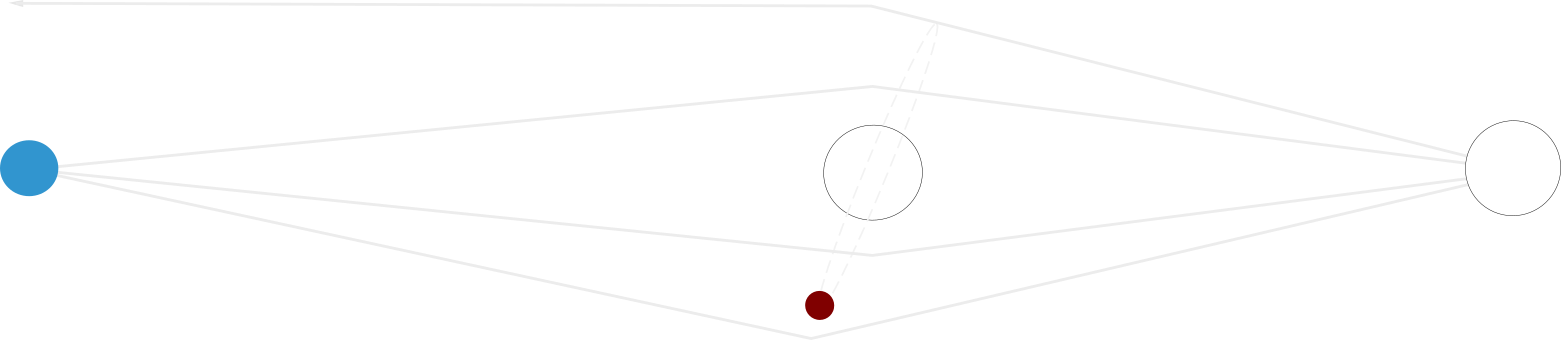
\includegraphics[width=12cm]{intro}
\caption{(self-drawn) schematic diagram of a microlensing event with an exoplanetary perturbation}
\label{fig:intro}
\end{figure}

These events are signified by a strong magnification spike of the background star as the two stars' angular separation minimizes over time.
The probability that two stars arrange themselves at any time for an observer to see noticeable effects is on the order of $10^{-6}$ (toward the Galactic bulge)\cite{gaudi}. 
However, in the last few decades with dedicated surveys using networks of telescopes, thousands of microlensing events have been observed.
Perhaps the motivation for ever-increasing efforts to find microlensing events is that
this phenomenon can be utilized as a tool for discovering extra-solar planets.
When there is a planet orbiting the lens star, if it is positioned correctly, it can further amplify the light-bending,
thereby yielding a spike in the magnification curve.
Considering the gravitational magnification as a deviation from a constant magnitude,
an exoplanetary detection can be thought of as a deviation from a deviation.

%Though this paper will discuss microlensing purely as a exoplanet detection method, gravitational lensing is a much wider subject area in astronomy and astrophysics.

% Gravitational microlensing for discovering exoplanets is unlike the other methods for exoplanet detection in many ways.
% Neither the lens star nor the planet have to be visible to witness the microlensing effects, so there is no need to search for events only in our local stellar neighborhood.
% Microlensing can peer into the planet populations of distant stellar neighborhoods as well as those of other galaxy's.
% \cite{martin}
% Microlensing relies on the convenient orbital positioning of the planet for its detection, not its orbital motion.
% Therefore, it can discover planets with orbital periods much longer than those discovered by something like transits or Doppler-wobbles.

As exciting and unique as gravitational microlensing is, it shares the core of the other three indirect methods (Doppler-wobbles, transits, and astrometric-wobbles) for finding exoplanets.
Namely, just as transits are based on deviations in star luminosity,
microlensing is based on a curious-enough deviation from an expected magnification curve.
Therefore, the reliablity of of exoplanet detection with gravitational microlensing is built on
a precise and understood photometry,
The goal of this paper is to explore the nature of the photometry's noise.

\section{The Model}

The following is a brief overview through the physics of gravitational microlensing to define the relevant terms.

Gravitational microlensing consists of three objects: the lens mass; an observer; and the light source.
A more symbolic representation of a microlensing event is shown in below in Figure \ref{fig:symb_mic}.

\begin{figure}[H]
\centering
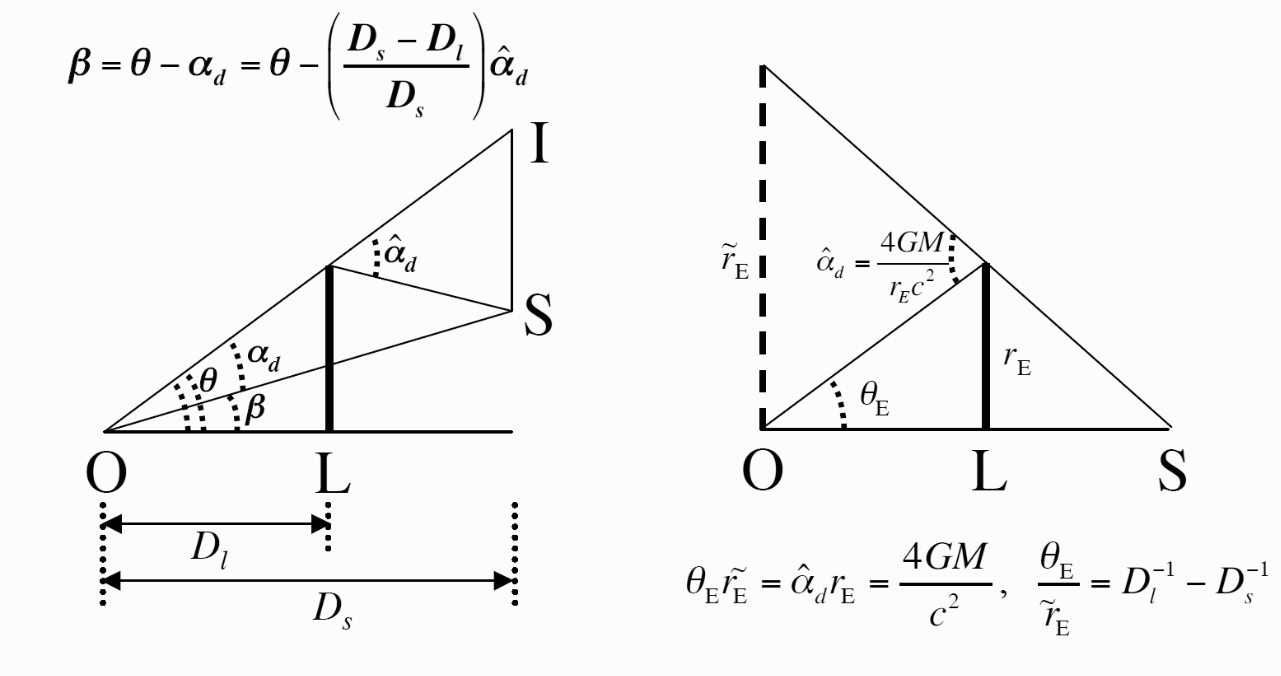
\includegraphics[width=15cm]{symb_mic}
\caption{(left) The lens \textbf{L} at a distance \textbf{D} from the observer \textbf{O}
  deflects light from the source \textbf{S} at distance $D_s$ by the Einstein bending angle $\hat{\alpha _d}$
 The angular positions of the images $\theta$ and unlensed source $\beta$ are related by the lens equation,
 shown in upper left.
 \newline (right) Relation of higher-order observables, the angular ($\theta _{\mathrm E}$) and projected ( $\tilde r_{\mathrm E}$) Einstein radii, to physical characteristics of the lensing system
(adapted from \cite{gaudi})
}
\label{fig:symb_mic}
\end{figure}

Unfortunately, in a discussion about precision, we hit the ground running with approximations.
Obviously relativity takes authority over Newton when discussing how gravity affects light, but an in-depth discussion of general relativity is beyond the scope of this paper.
Instead I will posit that for a point lens (an approximation of the star's finite but spherical symmetric size) the deflection angle is given by:
\[\hat \alpha _d = \frac{4GM}{c^2D_l\theta}\]
Where $M$ is the mass of the lens, and $\theta$ is the angular separation of the images of the source and the lens on the sky.\cite{gl_princ, gaudi}

The angular separation of the unlensed source and the lens $\beta$ is the angular separation between the image and the lens $\theta$ minus the angular separation of the image and the unlensed source $\alpha _d$. Further, with another approximation, $\hat \alpha _d(D_s-D_l)= \alpha _d D_s$. Therefore:
\[\label{eq1} \beta = \theta-\frac{4GM}{c^2\theta}\frac{D_s-D_l}{D_sD_l}\]

When the source is directly behind the lens ($\beta =0$), the source is imaged into an 'Einstein Ring'
\cite{gaudi}
with an angular radius:

\begin{equation}
\theta _\mathrm E =
\sqrt{\frac{4GM}{c^2}\frac{D_s-D_l}{D_sD_l}}
\qq{\arr} \beta = \theta - \frac{\theta _\mathrm E^2}{\theta}
\end{equation}

Next, we normalize all of the angles in terms of Einstein radii -- i.e. dividing both sides of [\ref{eq1r}] by $\theta _\mathrm E$
and defining 
$u=\beta /\theta _\mathrm E$ (describing the position of the source)
and $y=\theta /\theta _\mathrm E$ (describing the image(s) of the source)
This yields
$u=y-y^{-1}$
, which is equivalent to to the quadratic equation of
$y^2-uy-1=0$.
Therefore when the foreground star does not perfectly eclipse the background star ($u\neq 0$),
\[y_\pm = \pm \frac12\pqty{\sqrt{u^2+4}\pm u}\]
Thus, two images of the source are created that are typically stretched tangentially and compressed radially
\cite{gaudi} in terms of the Einstein circle.

In the plane of sky, the infinitisimal area of a source (imagined as a slice of a ring) is $\beta \ \mathrm d \beta \ \mathrm d \phi$ or $u \ \mathrm d u \ \mathrm d \phi$.
The area of the images is $\theta _\pm \ \mathrm d \theta _\pm \ \mathrm d \phi$ or $y \ \mathrm d y \ \mathrm d \phi$
for the same $ \ \mathrm d \phi$.\cite{gl_princ}
The concept of this magnification is better illustrated below in figure \ref{fig:symb_mag}

\begin{figure}[H]
\centering
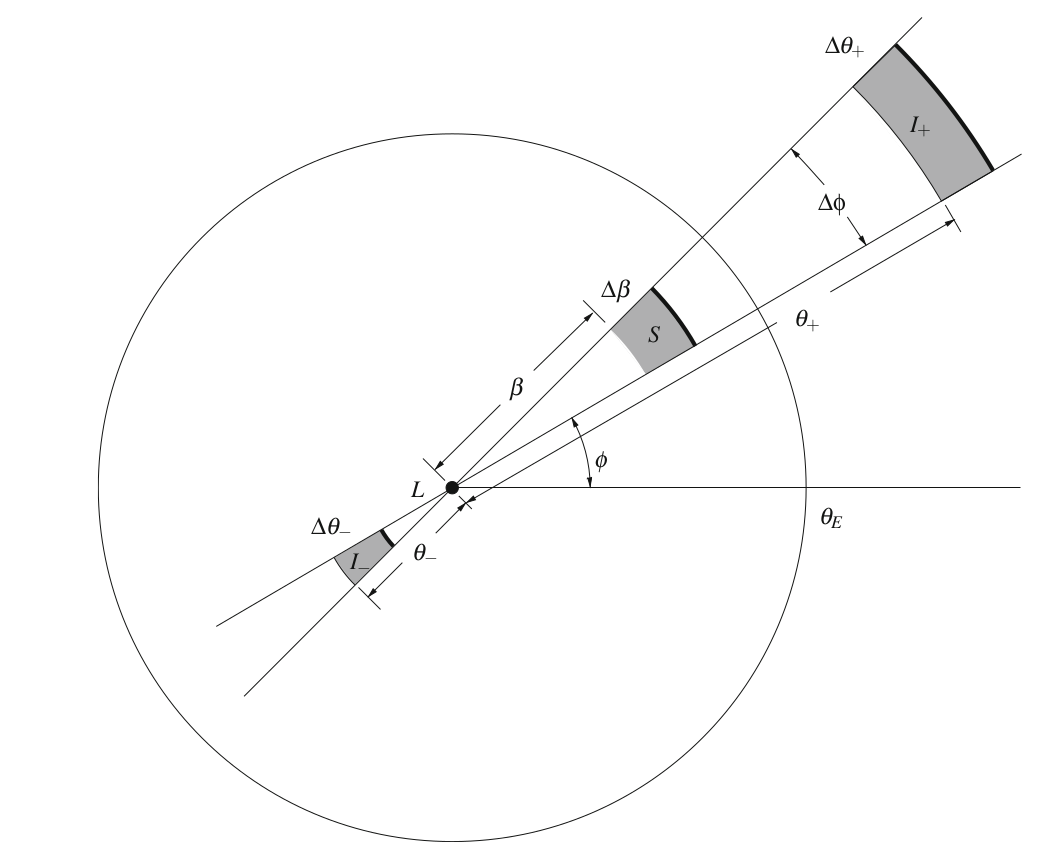
\includegraphics[width=12cm]{symb_mag}
\caption{
 In the plane of the sky, a source $S$ at angular distance
$\beta$ from lens $L$ appears as images $I_\pm$ at distances
$\theta _\pm$.
The angle $\phi$ is arbitrary.
The (infinitesimal) area of $S$ is $\beta\ \Delta \beta\ \Delta \phi$,
while that of $I_\pm$ is $\theta_\pm\ \Delta \theta _\pm \ \Delta \phi$
(adapted from \cite{gl_princ})
  }
\label{fig:symb_mag}
\end{figure}

Thus the ratio between the area of the image to the area of the source, the magnification (because surface brightness is conserved)
is: (exchanging the general $\theta$ and $\beta$ with our $y$ and $u$ respectively)
\[A_\pm = \abs{\frac{y_\pm}{u}\dv{y_\pm}{u}}
=\frac12\bqty{\frac{u^2+2}{u\sqrt{u^2+4}}}\]
And the total magnification considering both images is:
\[A(u)=\frac{u^2+2}{u\sqrt{u^2+4}}\]
with $u$ being the parameterized equation of the relative lens-source motion:
\[u(t)=\sqrt{u_0^2+\pqty{\frac{t-t_0}{t_\mathrm E}}^2}\]
where $u_0$ is the minimum separation between the lens and source, $t_0$ is the time of maximum magnification, and $t_\mathrm E$ is the timescale to cross the angular Einstein ring radius.

With this magnification in terms of the source motion, we have finally arrived at the simplest case of a microlensing event, also known as a Paczynski curve.\cite{gaudi}

Adding one more light deflector into this system like a planet dramatically increases the complexity of its optics -- so much so that the magnification curve is better looked at numerically and qualitatively rather than analytically.
% A multiple-lens system brings about magnification patterns that can't easily be described as images, or caustics, at certain source positions.
% They are paramaterized by the mass ratio $q$ of the lenses and their separation $d$.
% They are defined the set of source positions for which the magnification of a ponit source is formally infinite.
The bell-shaped prestinity of the Paczynski curve falls apart.

However, the important takeaway from this section is the Paczynski curve which can be used to better handle the microlensing data available.



\section{Photometry Data Modeled with Paczynski Curves}

Gravitational microlensing is a demanding task. It both requires a long, wide survey as to allow for the low probability of microlensing events to occur, and it requires precise photometry of the events when they happen (as each detection is likely the only glimpse of the properties of the planet that earth will ever get). So just like every other desire in astronomy, there are two goals to advance the power of gravitational microlensing: to increase both sampling rates and signal-to-noise ratios.

What is observed by the surveys searching for microlensing events in dense stellar fields is the flux of a photometered source as a function of time:
\[F(t)=F_sA(t; t_0, t_{\mathrm E}, u_0)+F_b\]
where $F_s$ is the flux of the source star, and $F_b$ is the flux from all of the light that is not being lensed.

So, $F(t)$ can be fit by five parameters: $t_0,u_0,t_\mathrm E,F_s,F_b$ which are highly correlated to eachother and only multiply when more lenses incorporate themselves into the picture.
A microlensing event with a planet involved is shown below in Figure
\ref{fig:phot_dat}. This data is taken from the OGLE-IV project \cite{ogle}

The OGLE project (Optical Gravitational Lensing Experiment) is a massive, long term, regular survey of the Magellanic Clouds and the Galactic Bulge (for maximum background stars)
The project is comprised of Polish and American astronomers based in the Las Campanas Observatory in Chile.
While the first phase of the OGLE project began in 1996, the fourth phase began in 2010 with a 32 chip masaic camera.
More information about the project can be found here \cite{ogle}.

\begin{figure}[H]
\centering
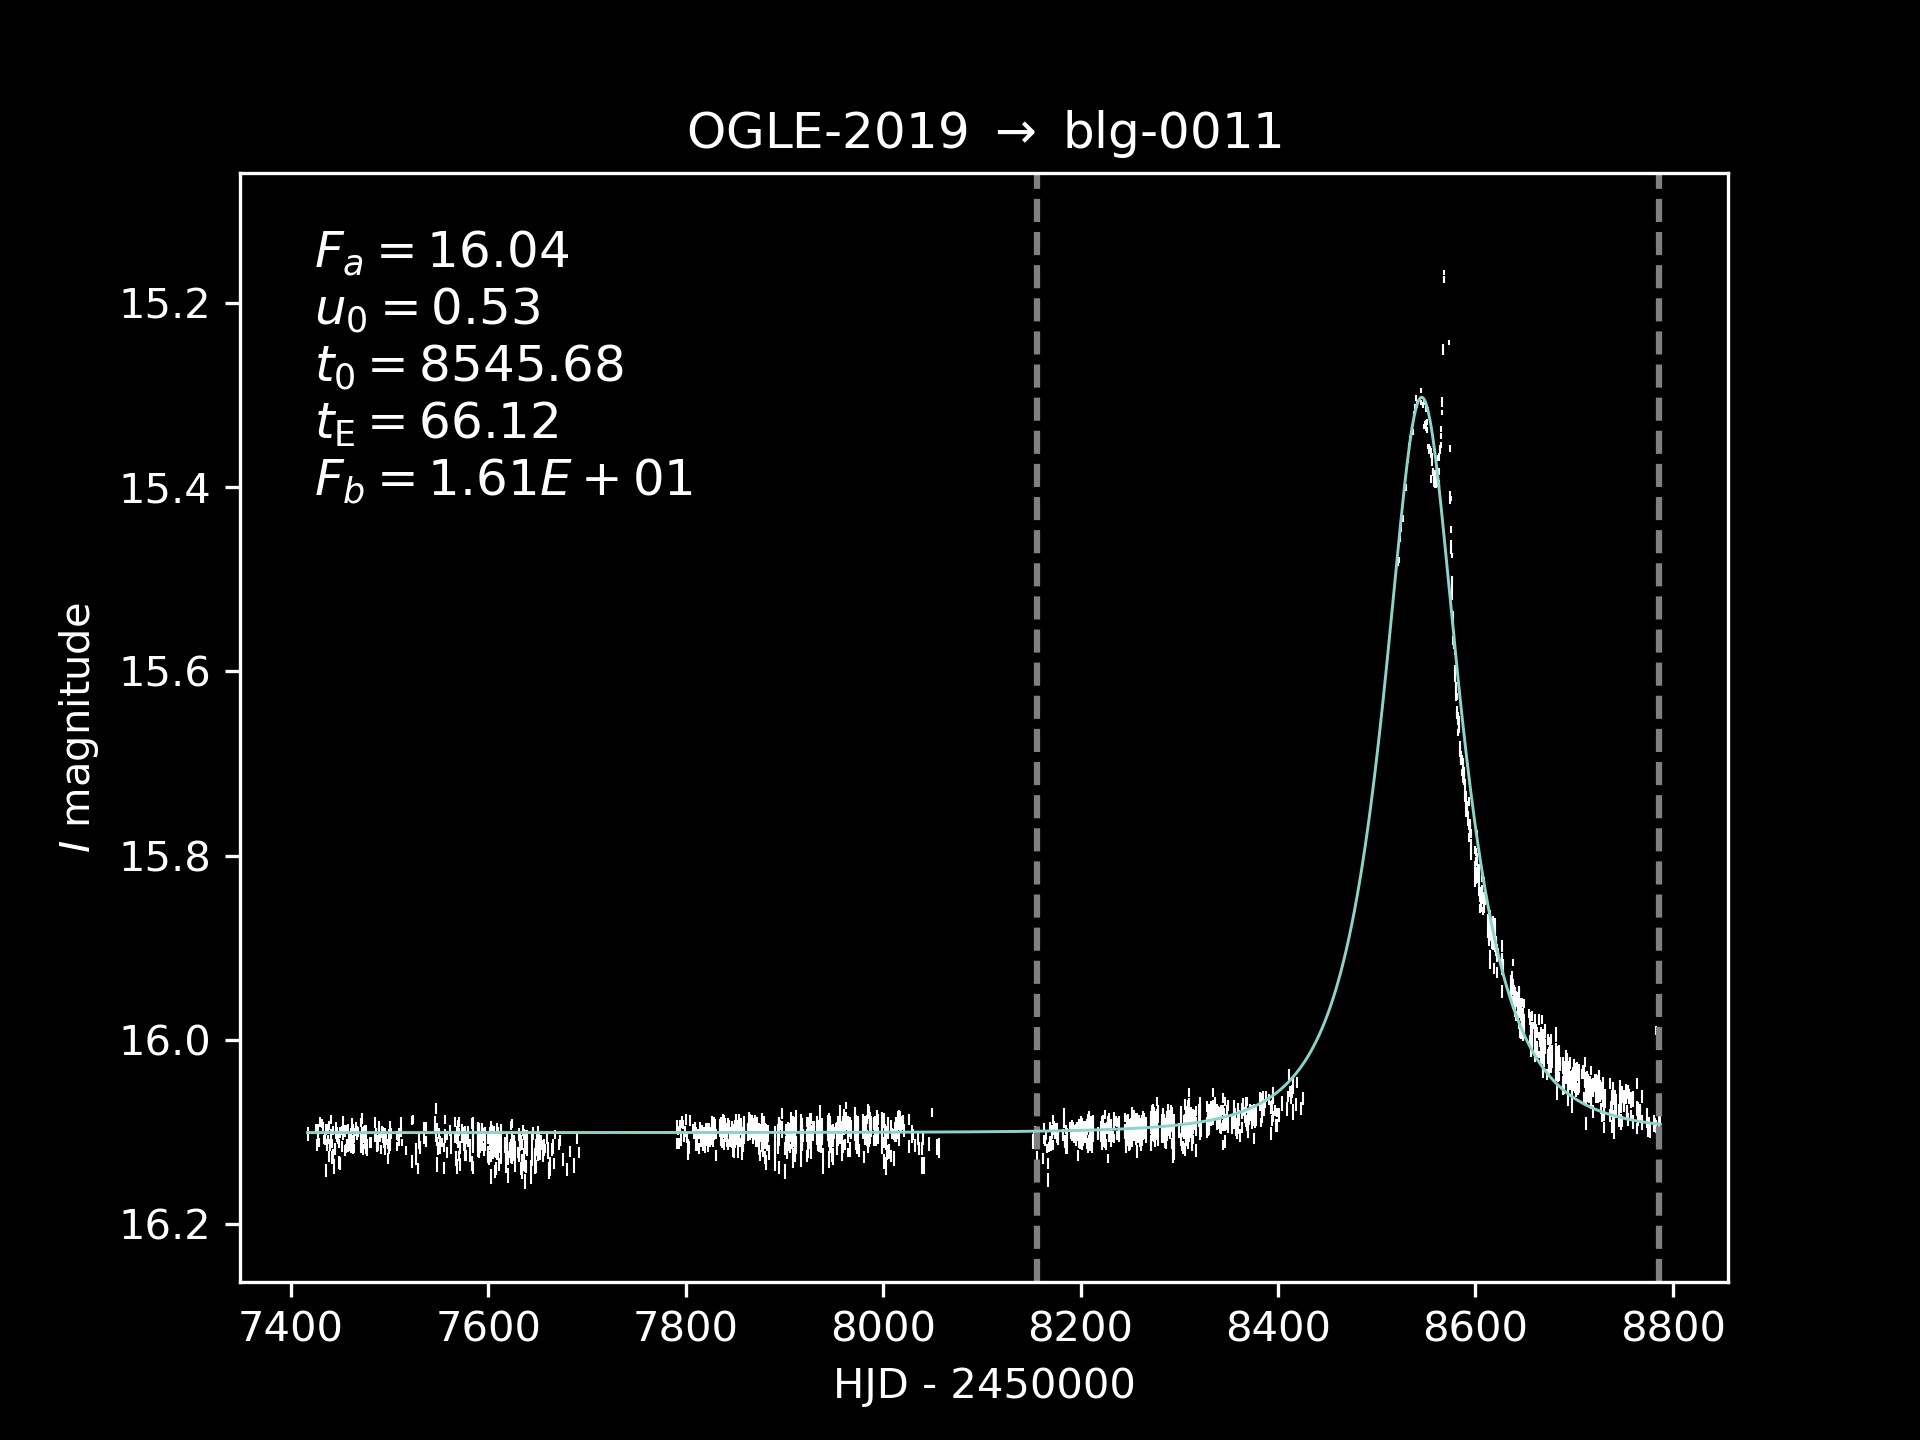
\includegraphics[width=\textwidth]{phot_dat}
\caption{Showing modeled magnitude measurements of a microlensing event in 2019.
  The small deviation in the peak is likely an exoplanet.
  Dashed lines isolate the magnification curve from the data.}
\label{fig:phot_dat}
\end{figure}

In order to characterize the validity of planetary perturbations, it should be necessary to explore the characteristics of this light curve where nothing is uncertain.
In other words the tail observing seasons where the flux measurement is constant should inform the statistical characterisics of the magnification curve.

\section{Data Distribution at Constant Brightness}
The priority of the description of this constant-brightness data is to understand the probability of \emph{certain} and \emph{significant} deviations from the mean.
Not only is it important to the validity of any statistical model's fit, but it is especially important in a detection method.

Taking the constant-brightness data at face-value, the distribution of magnitude measurements is shown below in Figure \ref{fig:freq_dist}

\begin{figure}[H]
\centering
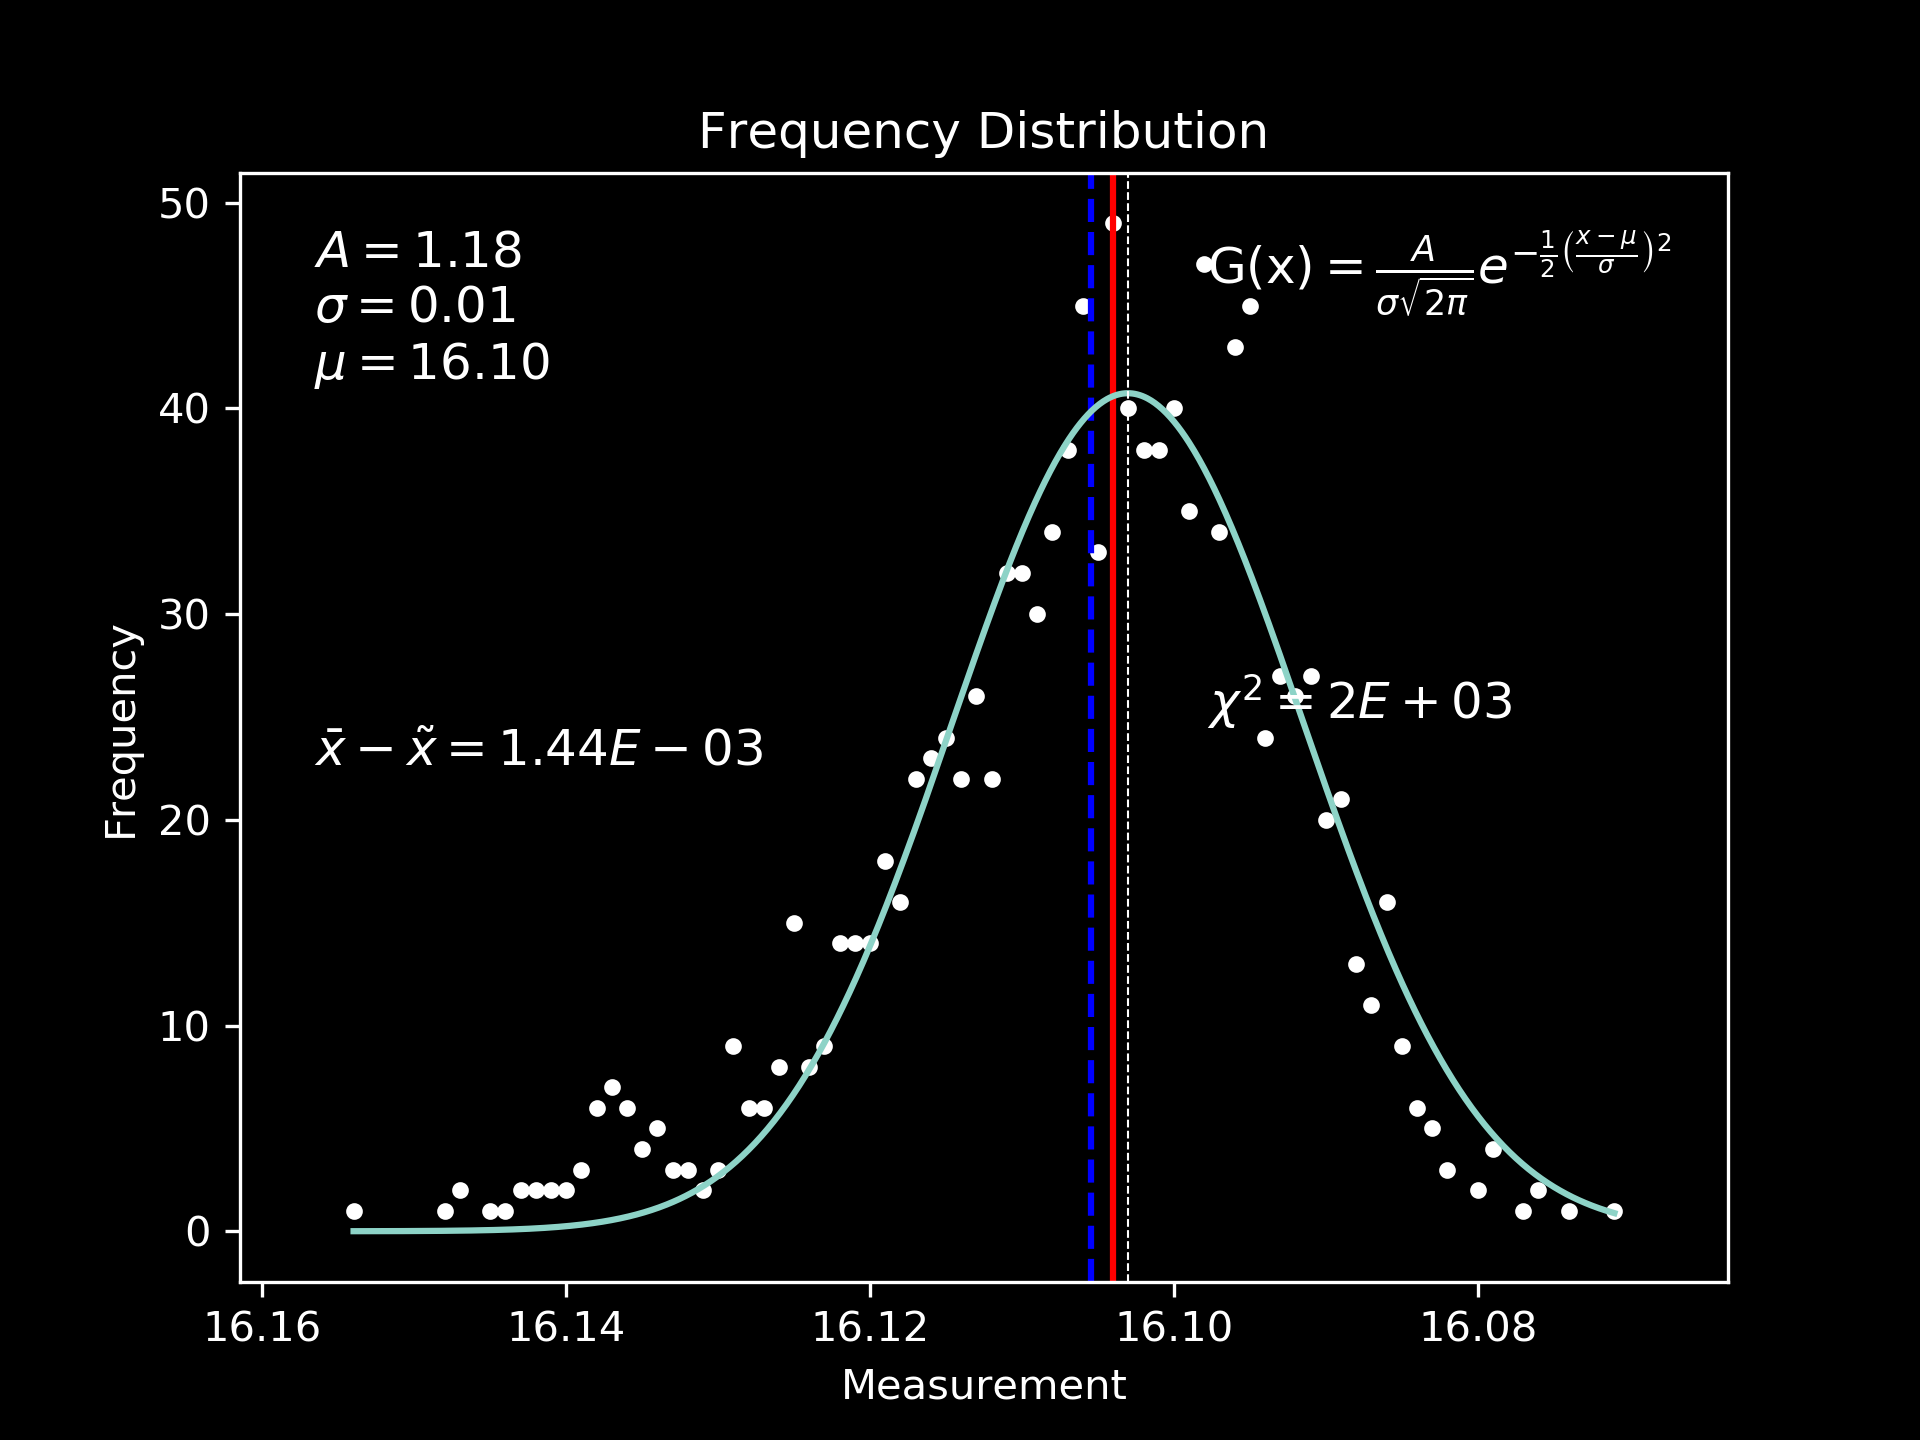
\includegraphics[width=\textwidth]{freq_dist}
\caption{This frequency distribution's only binning method is the digitization of its brightness measurements.
  \emph{i.e.} each 'bin' in this plot contains duplicate measurements resulting from the limited precision in the acquisition.
  Shown here is (left) the difference between the mean and the median measurement (in this case showing a right-skewed symmetry).
  The $\chi ^2$ statistic indicates a measure of `goodness-of-fit.'
}
\label{fig:freq_dist}
\end{figure}

Also shown is a Gaussian fit of this frequency distribution.
The Gaussian (or normal) probability density function is given by:
\[
f(x; \sigma, \mu)
= \frac{1}{\sigma\sqrt{2\pi}}
e^{-\frac12\pqty{\frac{x-\mu}{\sigma}}^2}
\]
Already an assumption has risen that this data follows a normal distribution, so is that a valid assumption to make?
Already we observe outliers in the data that does not follow the Gaussian fit in this constant-brightness data.

As shown in Figure \ref{fig:phot_dat}, the OGLE data has inherent reported errors.
Aligning this analysis with the first piority, we incorporate each measurement's uncertainty into the distribution by instead measuring the distribution of residuals:

\begin{equation}%{\label{ress}}
% \mathcal{R} = \vqty{\frac{x - \bar x}{\Delta x}}\]
\mathcal{R} = \frac{x - \bar x}{\vqty{\Delta x}}
\end{equation}

$\mathcal{R}$ illustrates that the focus of the fit is proportional to each measurement's deviation from the mean
 $\mathcal{R} \sim x-\bar x$
and inversely proportional to the level of uncertainty/error
$\mathcal{R} \sim (\Delta x)^{-1}$.
Introducing this definition dramatically broadens the range of possible values, thereby increasing the density of the measurement axis of a frequency distribution.
Rather than bin the data, we look at the constant-brightness-deviation data's emprical cumulative distribution function (CDF):
\[ F(x) = P(X \leq x) \]

Such a CDF of our present example photometry data is shown below in Figure \ref{fig:cumu_dist}.
Putting the CDF equation into words, the CDF measures what fraction of the data is less than a given data point.
Because the $y$-axis can be thought of as how much of the distribution is underneath a measurement, the upper region of the CDF is of particular interest.
The cumulative distribution function of a statistical model can be solved analytically. For example, the CDF of a Gaussian model is given by:
\begin{equation*}
\begin{aligned}
F_{\mathrm G}(x) &= \int_{-\infty}^x f_{\mathrm G}(t)\ \dd t
\\&= \frac{1}{\sqrt{2 \pi}}
\int _{-\infty}^x e^{-\frac{t^2}{2}}\ \dd t
\\ F_{\mathrm G}\pqty{\frac{x-\mu}{\sigma}}
&= \frac{1}{\sqrt{2 \pi}}
\int _{-\infty}^u e^{-\frac{t^2}{2}}\ \dd t
\qquad
u(x) = \frac{x-\mu}{\sigma}
\qquad
x = \mathcal{R}
\end{aligned}
\end{equation*}

A fitted Gaussian CDF is shown below in Figure \ref{fig:cumu_dist}.

\begin{figure}[H]
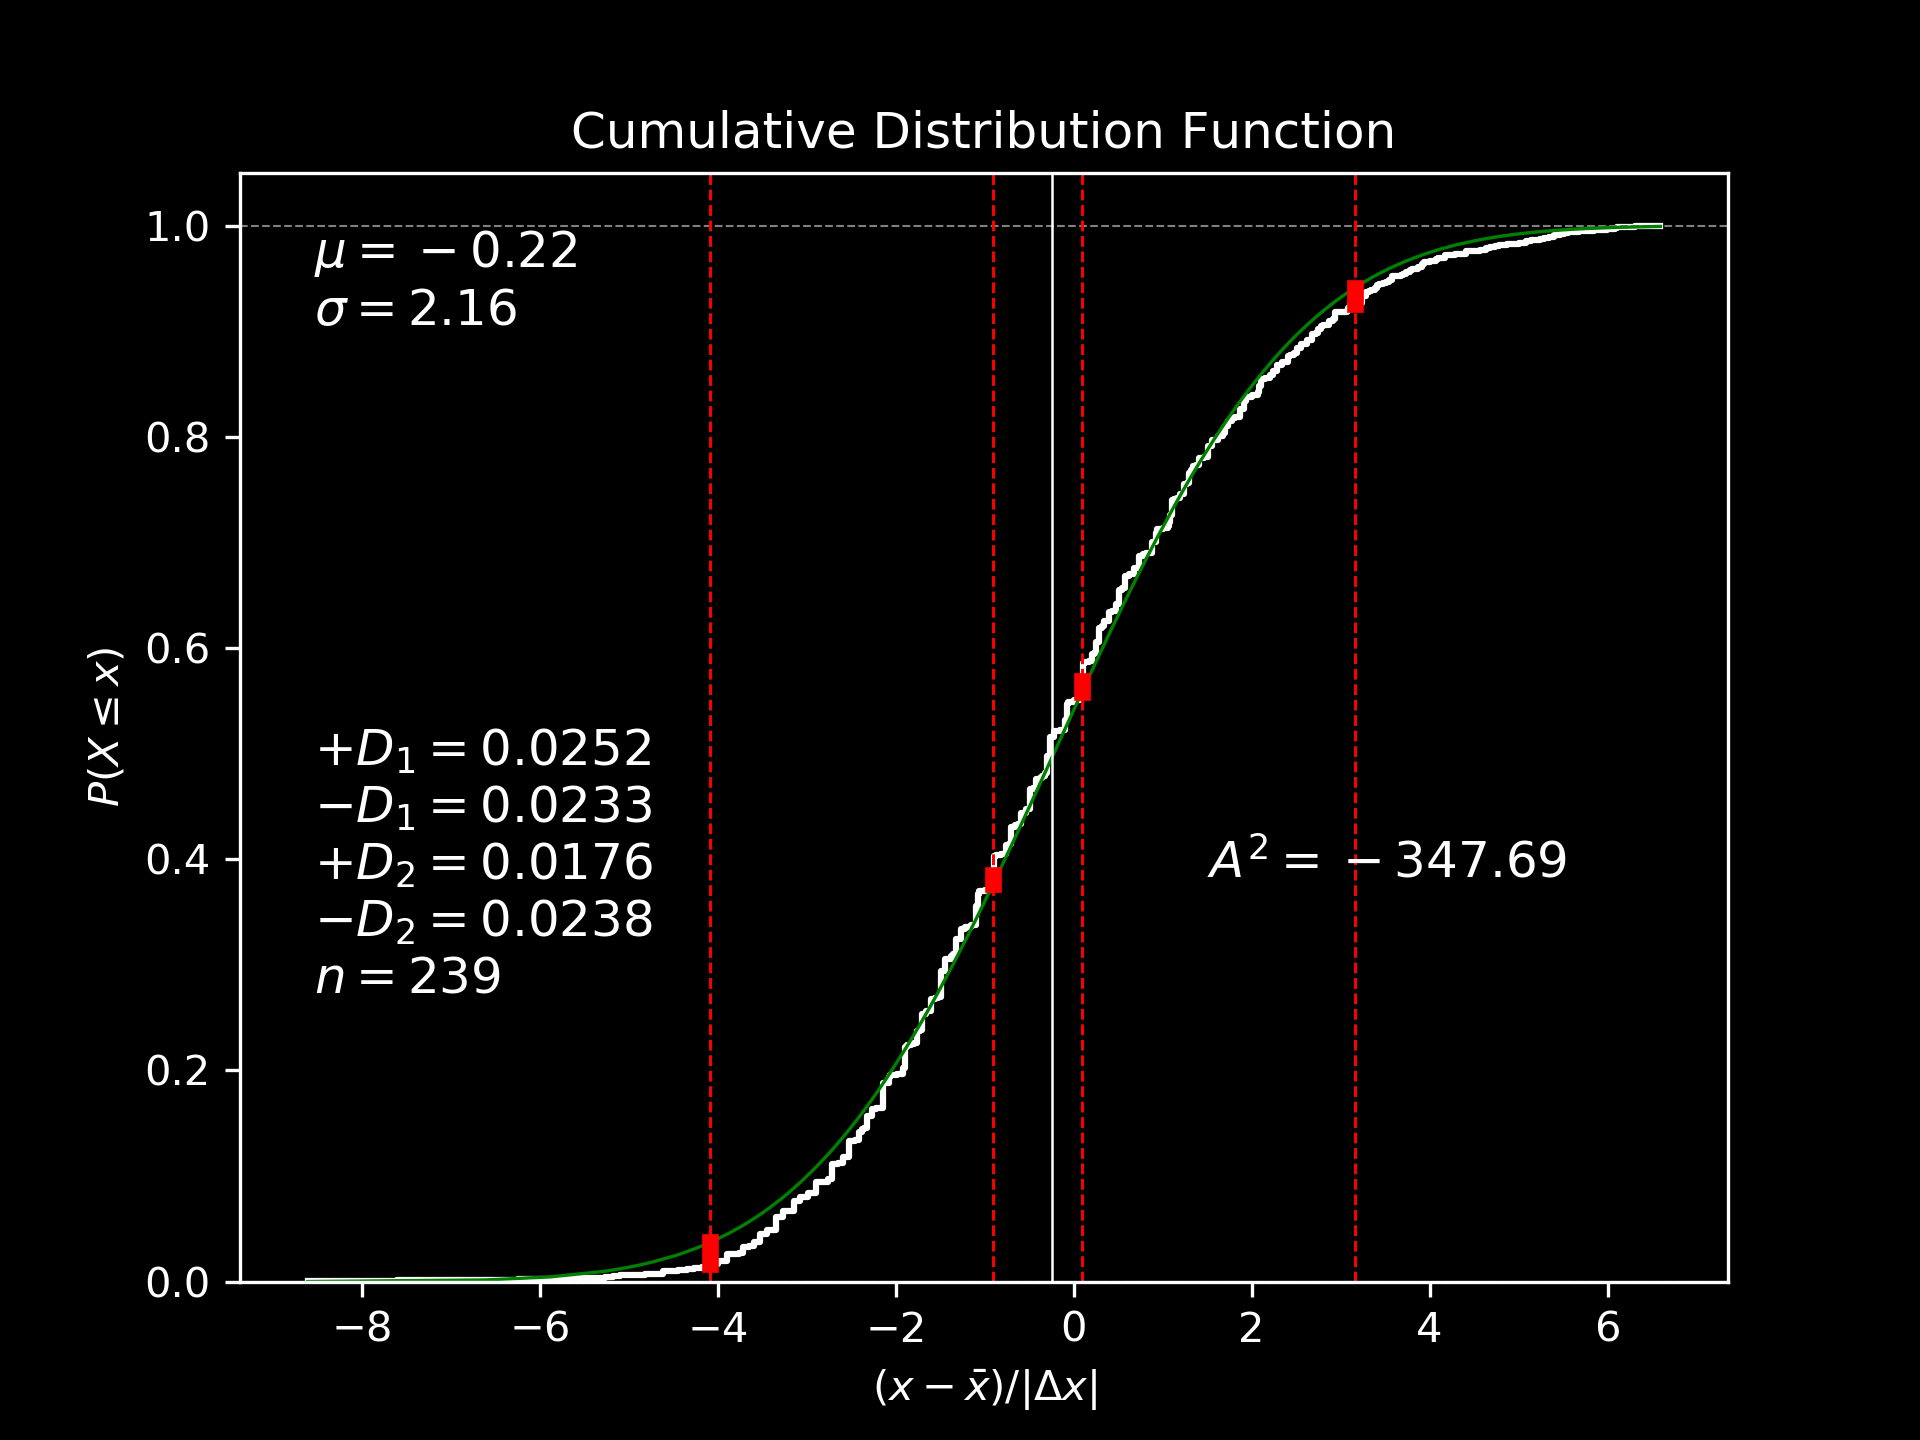
\includegraphics[width=\textwidth]{cumu_dist}
\centering
\caption{Shown here is the CDF of the $\mathcal{R}$ data.
  Mapped onto it is a paramaterized normal CDF with two tests: the Kolgomorov-Smirnoff test (the $\pm D_i$ and red lines) and the Anderson-Darling test ($A^2$).
  $n$ is the number of measurements.
  The black line is the inflection point of the model (which is eqiuvalent to $\mu$).
  (Note we have switched the example event to \texttt{blg-0040})
}
\label{fig:cumu_dist}
\end{figure}

Rather than the usual Kolgomorov-Smirnoff test (KS-test),
which is the maximum difference between the two CDFs,
I have given the test four prongs to measure each aspect of the CDF difference:
\begin{enumerate}
\item $+D_1$ maximum difference between model and eCDF before the center value 
\item $-D_1$ maximum difference between eCDF and model before the center value 
\item $+D_2$ maximum difference between model and eCDF after the center value 
\item $-D_2$ maximum difference between eCDF and model after the center value 
\end{enumerate}

Again, two of these four values represent a deviation from the two tails of the eCDF, which are the focus of the test.
The critical values for the most part supercede the maximum of $D_i$, so it is better used as a way of comparing modified distributions.

Similarly, the Anderson-Darling statistic is mostly made as a comparison value among attempted fits, and it is calculated by:
\[
A^2 = -n - S
\qquad
S = \sum _{i=1}^{n}\frac{2i-1}{N}
\left[\ln(F(\mathcal{R})) + \ln(1-F(\mathcal{R}_{n+1-i}))
\right]
\]

Nevertheless, the quick fall-off of the normal distribution again becomes apparent;
the model approaches the 100\% assymptote before the data does. 
So how can one account for this discrepancy?
There are two approaches to ensure that the model distribution of the deviations does not overlook the non-zero probability of the tail:
\begin{itemize}
\item First is to expand the reportoire of model distributions with heavier tails.
Ideally this will yield a more shallow CDF assymptote.
\item Then, we add to the errorbar data in quadrature to steepen the data's CDF assymptote
\end{itemize}

\section{Heavy-Tailed Distributions}

The choice heavy-tailed distributions to add to this picture include the \textbf{student $t$-distribution} and the \textbf{Cauchy distribution}
They are both symmetric, so they can be utilized for measurement axes besides $\mathcal{R}$.

\subsection{Student's $t$-distribution}

The student's $t$-distribution was built upon the $t$-test to estimate the mean of a sample size that is too small, with an unknown standard deviation.
Obviously, the constant-brightness data is far from small, but because of its function to acommodate standard deviation uncertainty, it will prove useful for the task of accomodating data tails.
The probability density function of a $t$-distribution is given by:
\[
f(t; t_0, \nu) = \frac{1}{\sqrt{\nu}\ \mathrm{B}(\frac12, \frac{\nu}{2})}
\left( 1+\frac{(t-t_0)^2}{\nu}\right)^{-\frac{\nu+1}{2}}
\qquad
\mathrm{B}(x,y) = \int_0^1t^{x-1}(1-t)^{y-1}\ \dd t
\]
where $\nu$ is the number of degrees of freedom, and $\mathrm{B}(x,y)$ is the beta function.
We have also introduced $t_0$ to allow for the distribution to be non-central.
$t$-distributions with multiple degrees of freedom are shown below in Figure \ref{fig:t_dist}.

\begin{figure}[H]
\centering
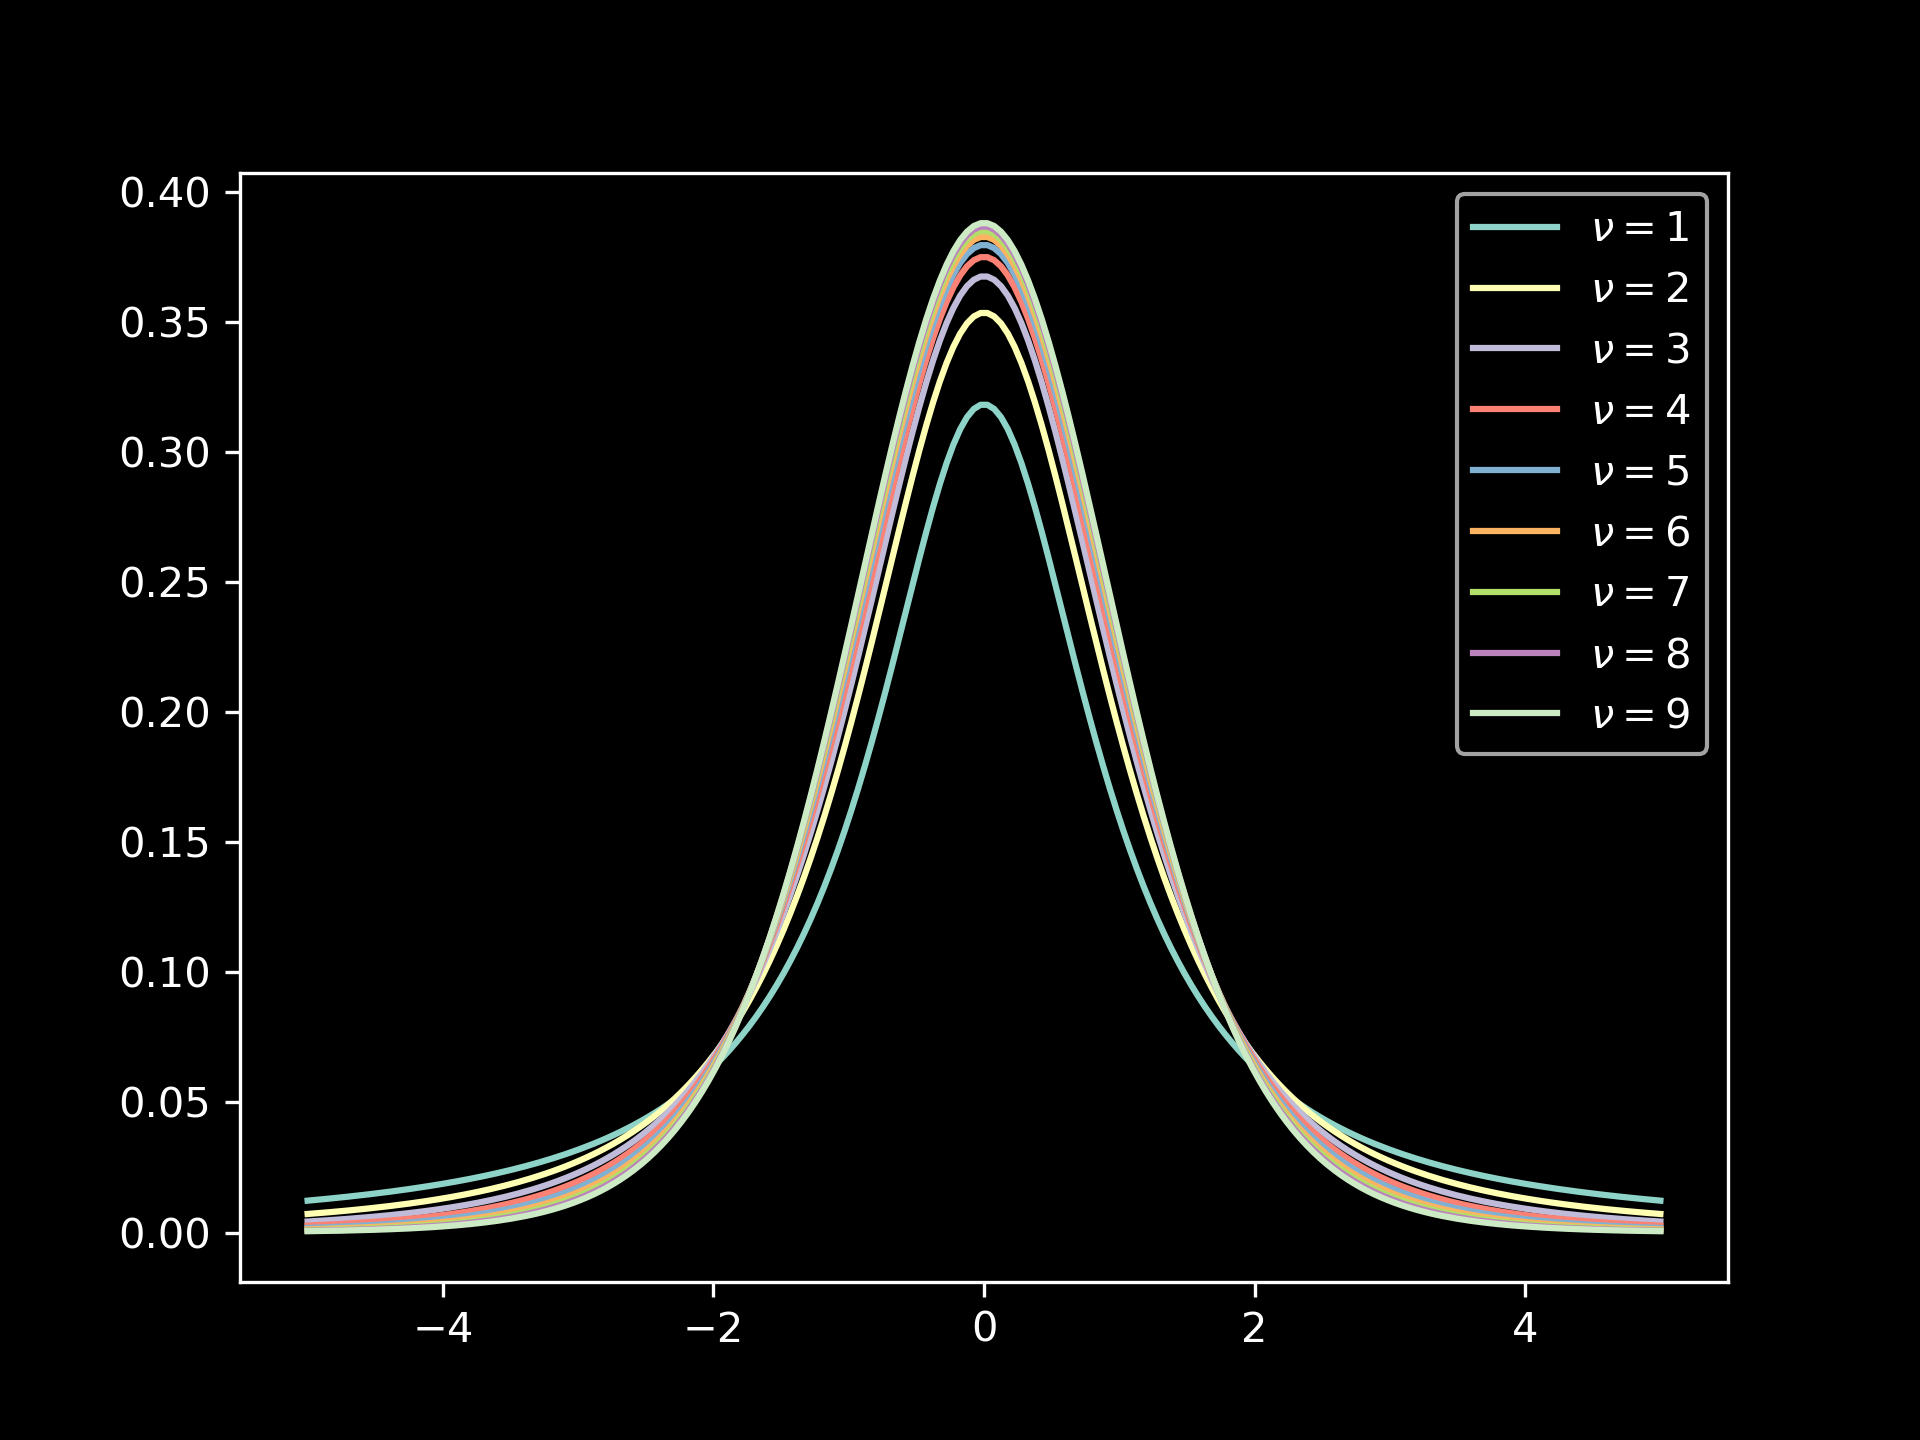
\includegraphics[width=8cm]{t_dist}
\caption{Model $t$-distributions centered at $t_0=0$. When $\nu=1$ is when this distribution is at its furthest from the normal distribution, which it converges to quickly.}
\label{fig:t_dist}
\end{figure}

With low $\nu$, the $t$-distribution posseses a smaller peak, and heavier tails.
As $\nu \rightarrow \infty$ the distribution approaches that of a normal distribution.
So in a way, the degrees of freedom can be measure of the deparature from a normal distribution.

Unfortunately, there seems no way to analytically simplify the $t$-distribution's CDF from the starting point: (which makes the CDF a computational nightmare)
\begin{equation*}
\begin{aligned}
F(t; u_0, \nu) &= \int_{-\infty}^tf(u)\ \dd u
\\&= \int_{-\infty}^t
\frac{1}{\sqrt{\nu}\ \mathrm{B}(\frac12, \frac{\nu}{2})}
\left( 1+\frac{(u-u_0)^2}{\nu}\right)^{-\frac{\nu+1}{2}}
\ \dd u
\end{aligned}
\end{equation*}

Now, the Figure \ref{fig:t_cdf} below shows the CDFs of the constant-brightness data and the CDFs of both a normal distribution and a $t$-distribution.

\begin{figure}[H]
\centering
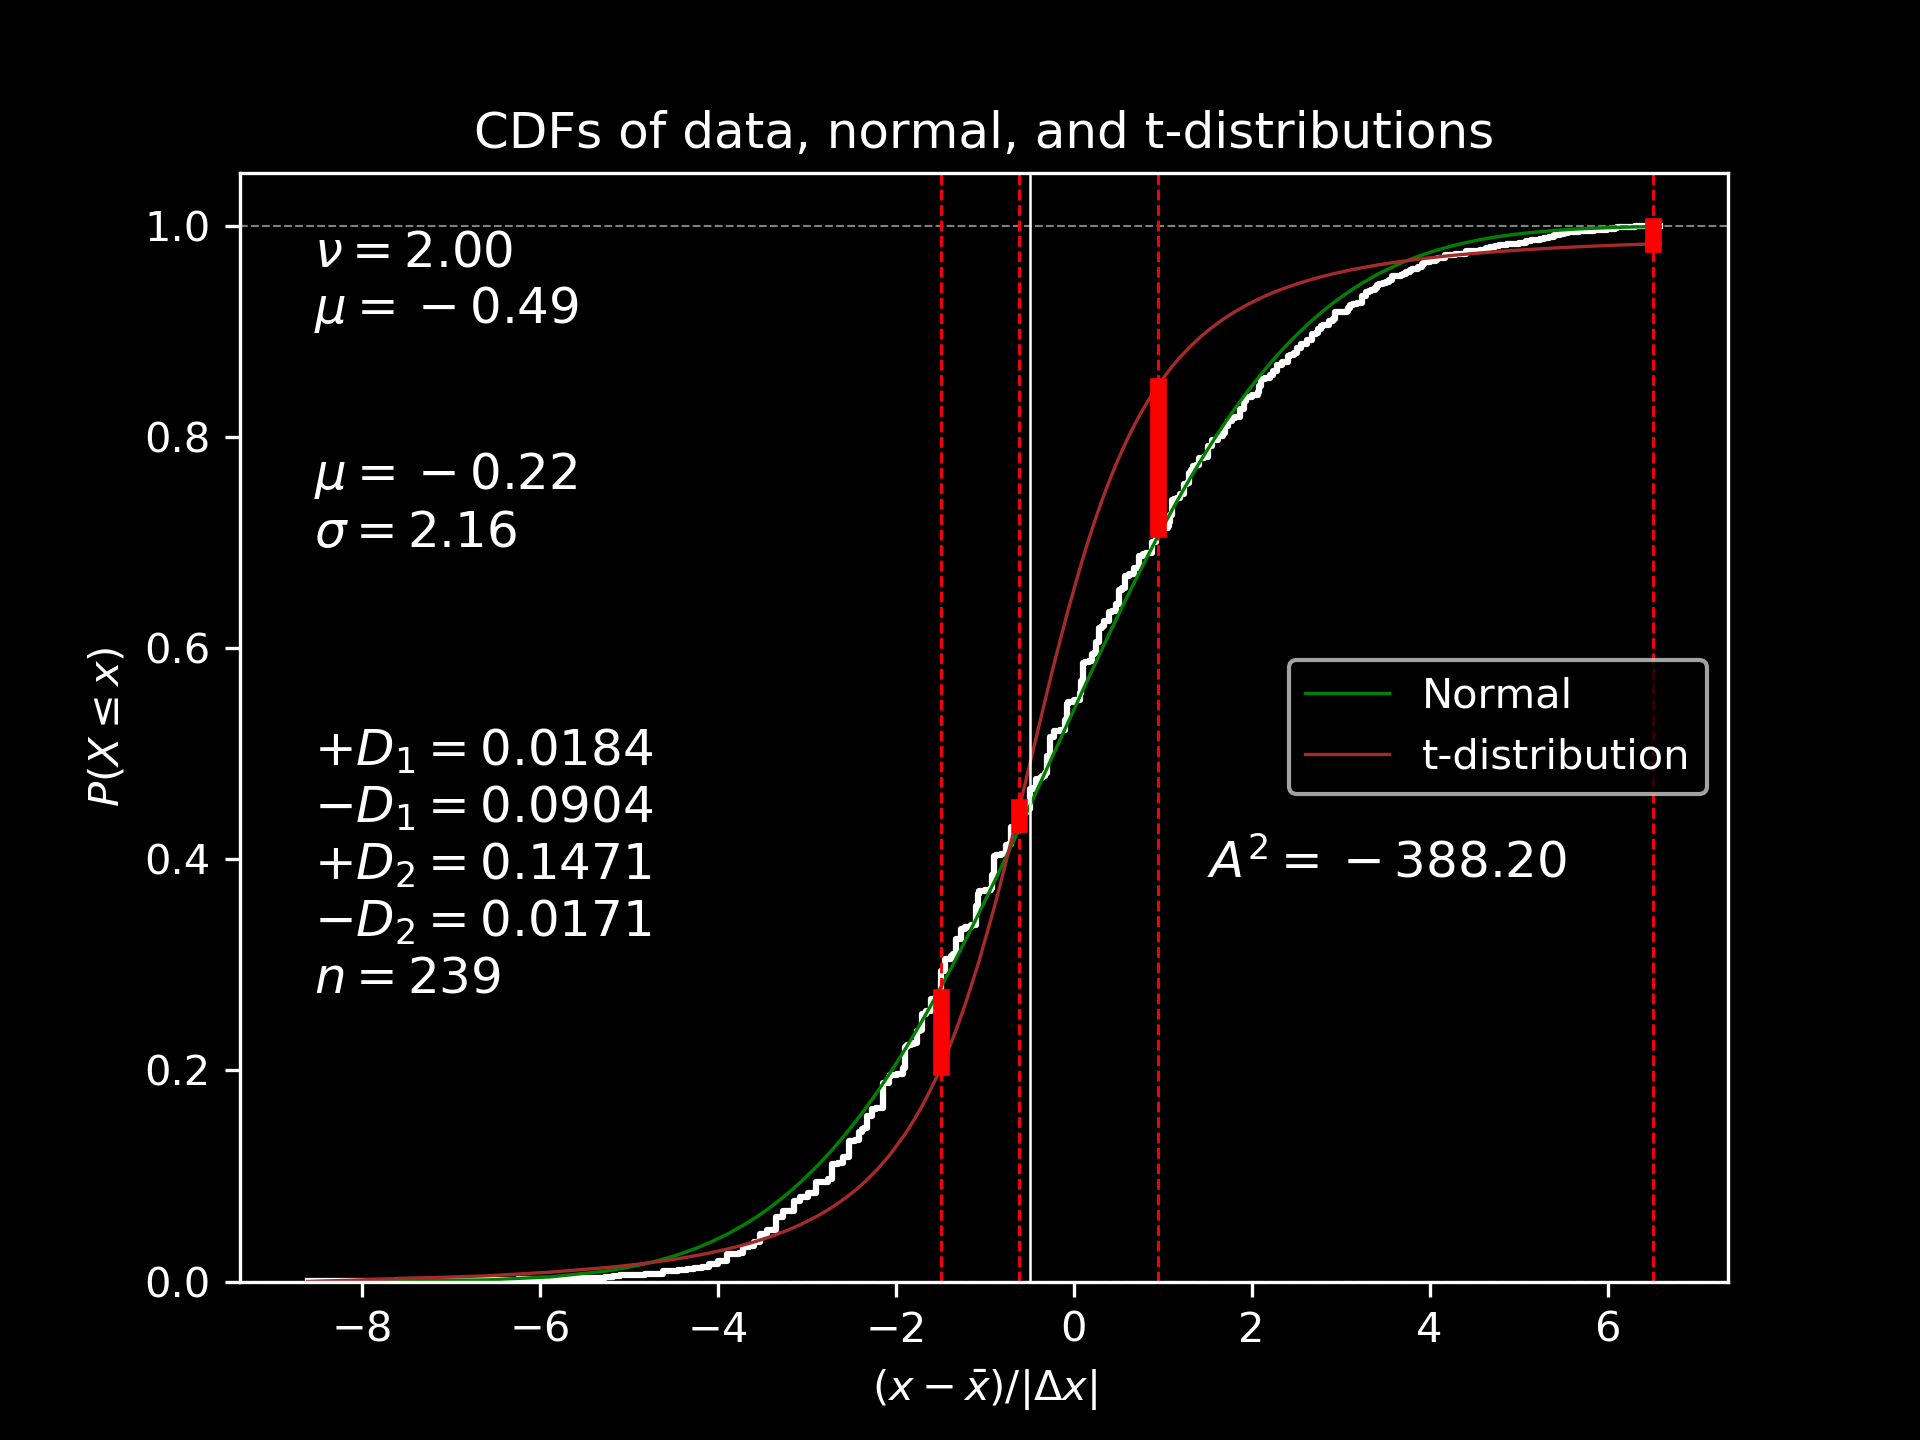
\includegraphics[width=\textwidth]{t_cdf}
\caption{The $t$-distribution is the one being tested.
  It performs worse on its `central' KS-tests, but its tails clearly stay within the bounds that our priority subjects the model CDF to.
}
\label{fig:t_cdf}
\end{figure}

\subsection{Cauchy distribution}

The Cauchy/Lorentz distribution has an old, (and controversially-named) history.
More importantly, this distribution is paramaterized by its full width at half maximum (FWHM) rather than its variance, and has much heavier tails than that of a normal distribution.

The Cauchy distribution is one of the few whose probability density function (and cumulative distribution function) can be expressed analytically:
\[
f(x; x_0, \gamma)
=\frac{1}{\pi\gamma}\left[1+\pqty{\frac{x-x_0}{\gamma}}^2\right]
=\frac{1}{\pi\gamma}\left[\frac{\gamma ^2}{(x-x_0)^2+\gamma ^2}
\right]
\]

\begin{figure}[H]
\centering
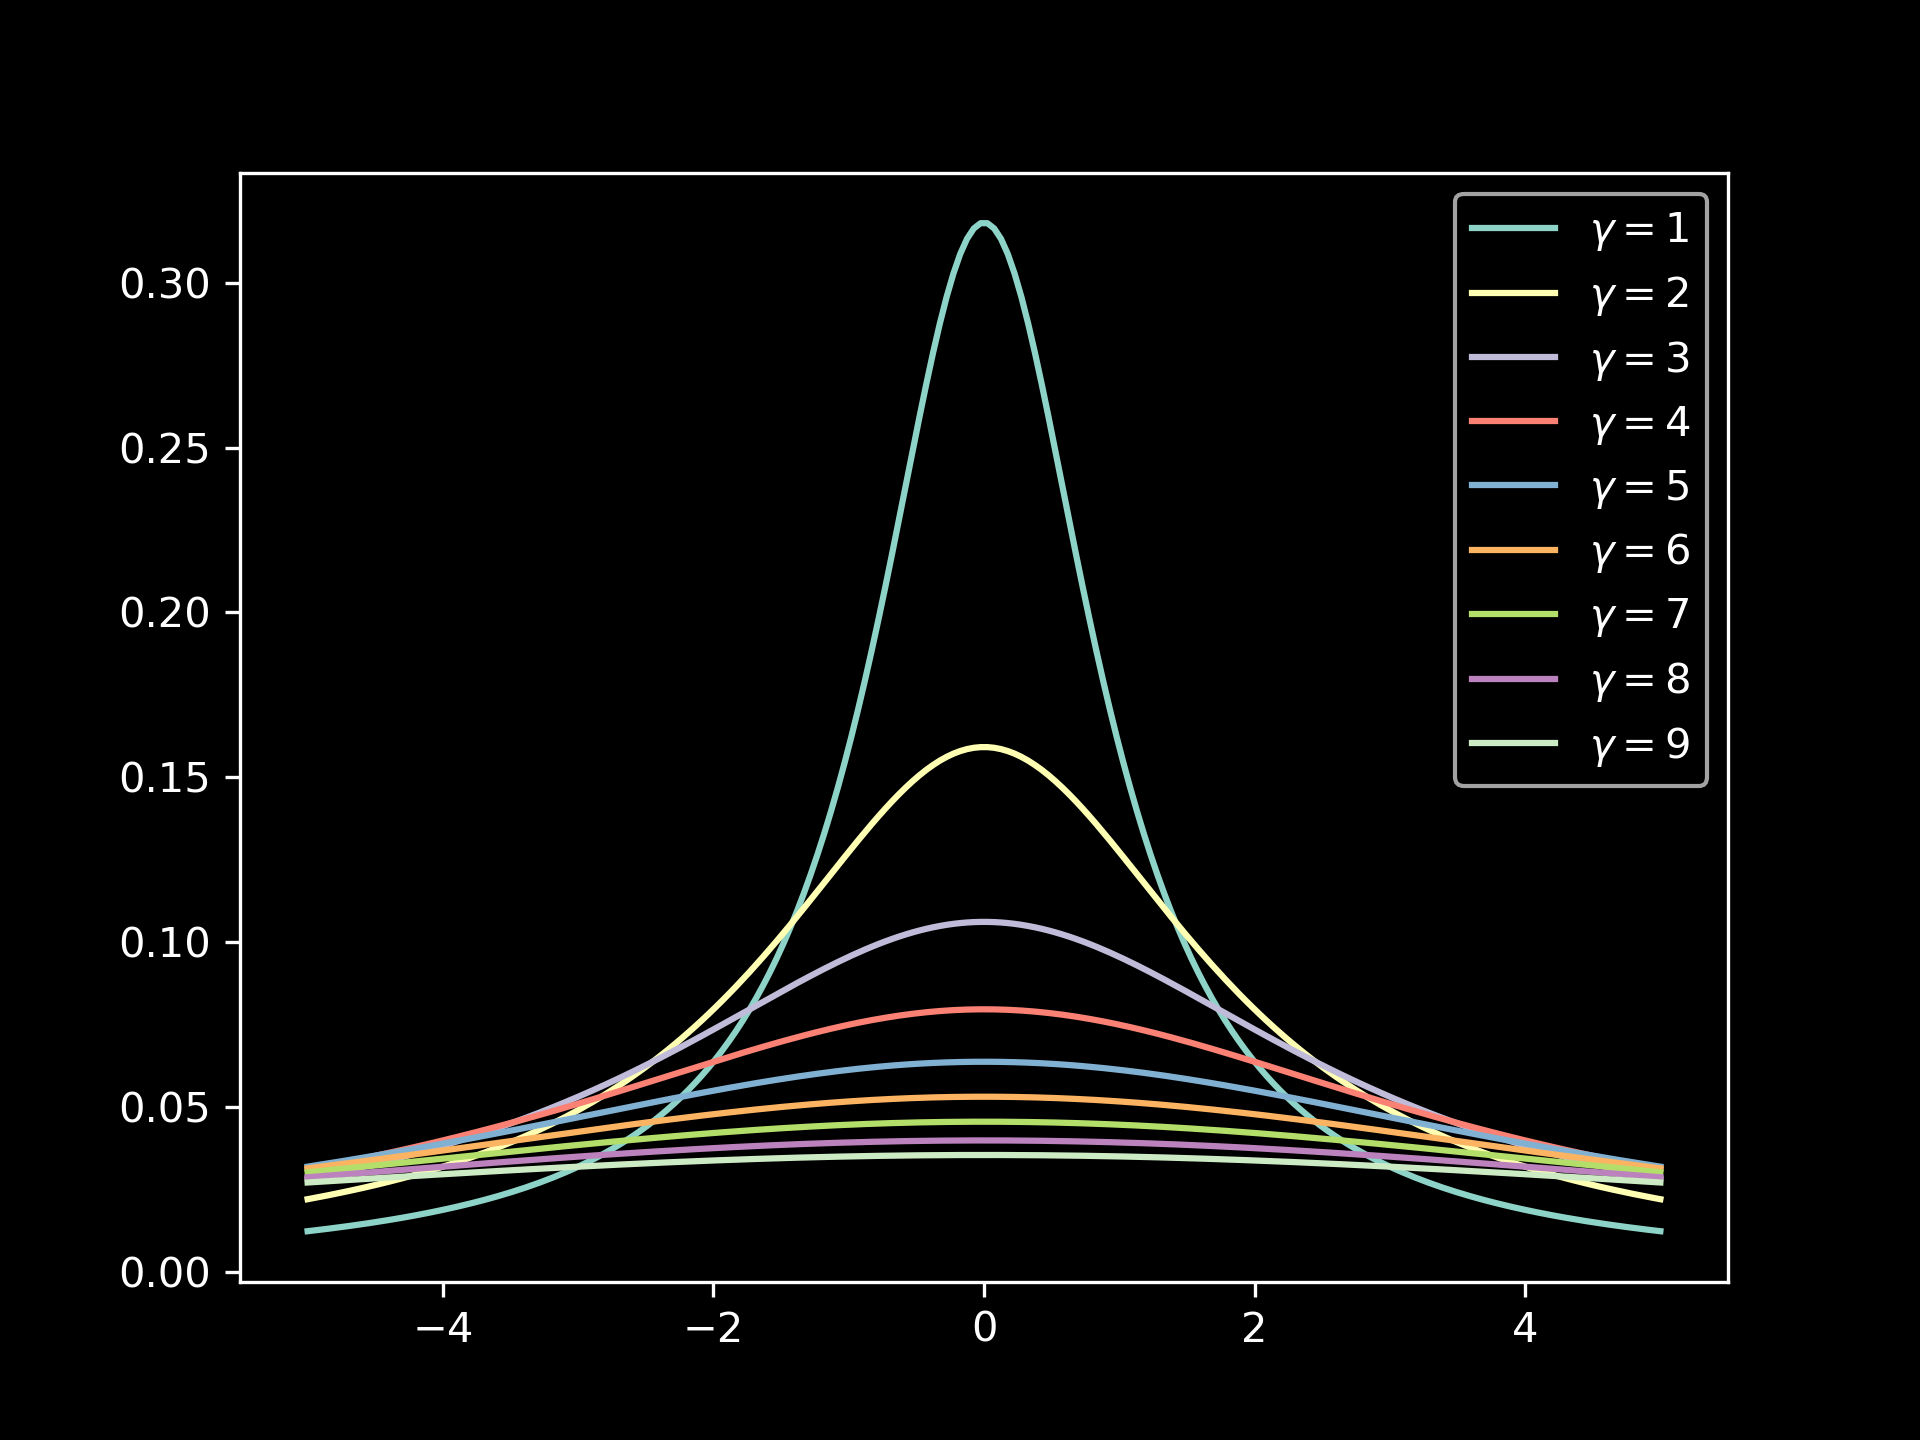
\includegraphics[width=8cm]{lo_dist}
\caption{model Cauchy/Lorentzian distributions centered at $x_0=0$ with increasing $ \mathrm{FWHM = 2\gamma$}}
\label{fig:lo_dist}
\end{figure}

Thus, the Cauchy CDF is given by:

\begin{equation*}
\begin{aligned}
F(x;x_0, \gamma) &=
\int _{-\infty}^x f(t)\ \dd t
\\&=\frac{1}{\pi}
\arctan\pqty{\frac{x-x_0}{\gamma}}+\frac12
\end{aligned}
\end{equation*}

The constant-brightness CDF, along with a Cauchy CDF and a normal CDF, is shown below in Figure \ref{fig:cauchy_cdf}.

\begin{figure}[H]
\centering
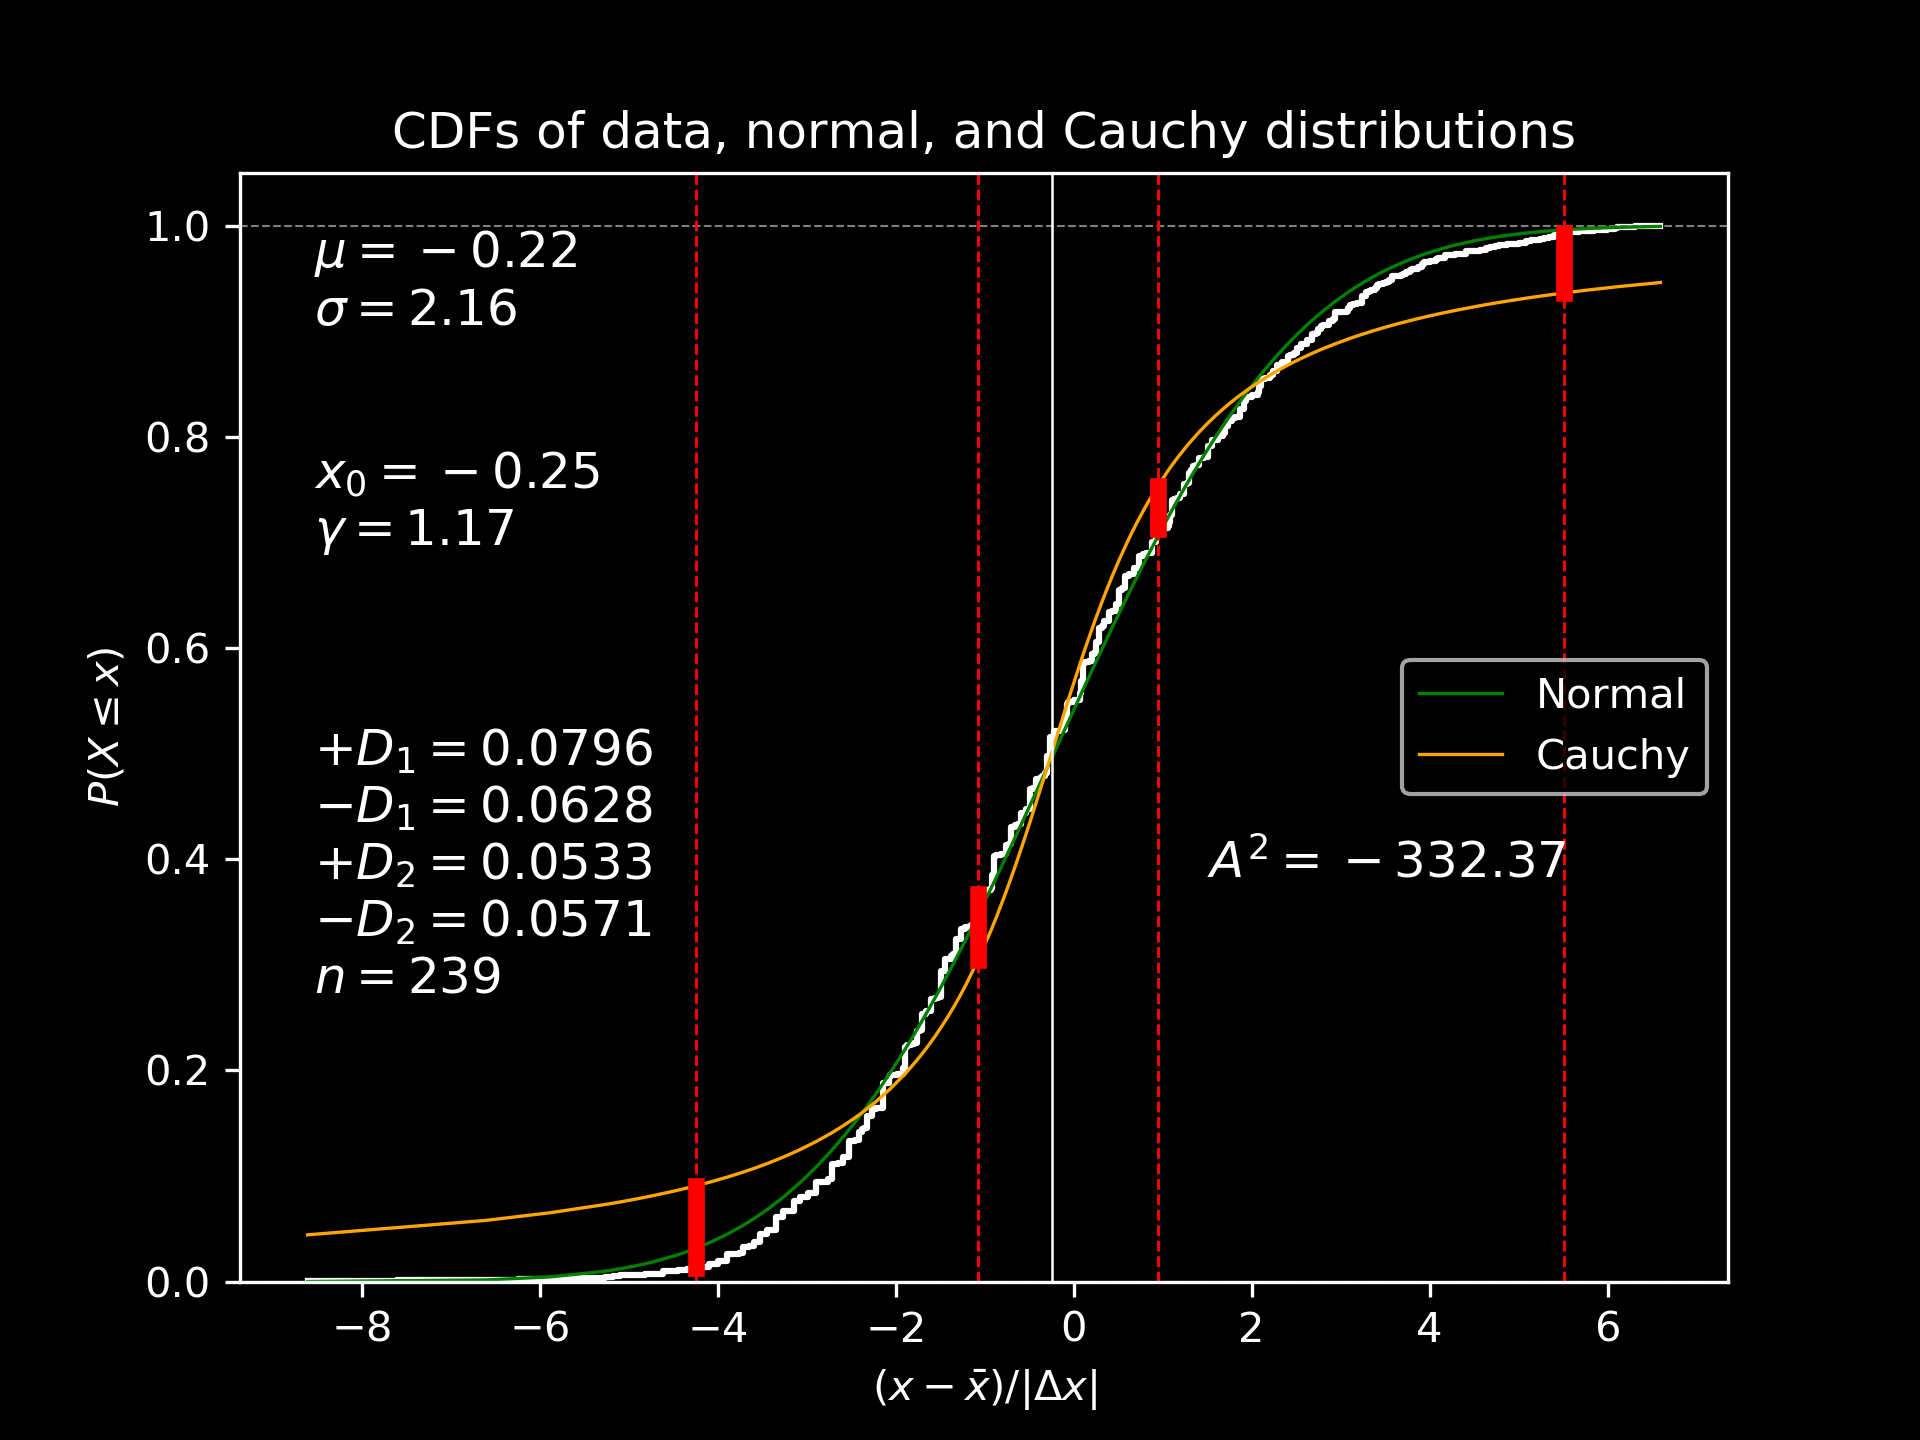
\includegraphics[width=\textwidth]{cauchy_cdf}
\caption{The Cauchy-distribution is tested.
  Similar to the $t$-distribution, it performs worse on its tests, but its tails are significantly well within 0 and 1.
  $+D_1$ and $-D_2$ are therefore boastfully high in this case.
  But priority one must not distract from priority zero which is to obtain a good fit in the first place.
  At what cost do we vertically compress our CDFs in this way?
}
\label{fig:cauchy_cdf}
\end{figure}


% \pagebreak
\section{Error Correcting}

These other distributions provide heavy tails, but as shown from the tests that we have subjected them to, perhaps the more accuracy-focused approach is to fine tune the normal distribution's fit.

The additional parameter to introduce is a correction to the uncertainty in the measurements.
Flatly increasing $\Delta x$ would narrow the probability density function of $\mathcal R$ and would therefore steepen the empirical cumulative density function.
Adding errors together follows Pythagorean error propagation rules, so we increase $\Delta x$ by:
\[
\Delta x \rightarrow \sqrt{\Delta x^2 + C^2}
\qq{so that}
\mathcal{R} = \frac{x-\bar x}{\sqrt{\Delta x^2 + C^2}}
\]

Shown below in Figure \ref{fig:err_cor1} are the CDFs of both the original dataset and the dataset where
$\Delta x \rightarrow \sqrt{\Delta x + 0.1}$

\begin{figure}[H]
\centering
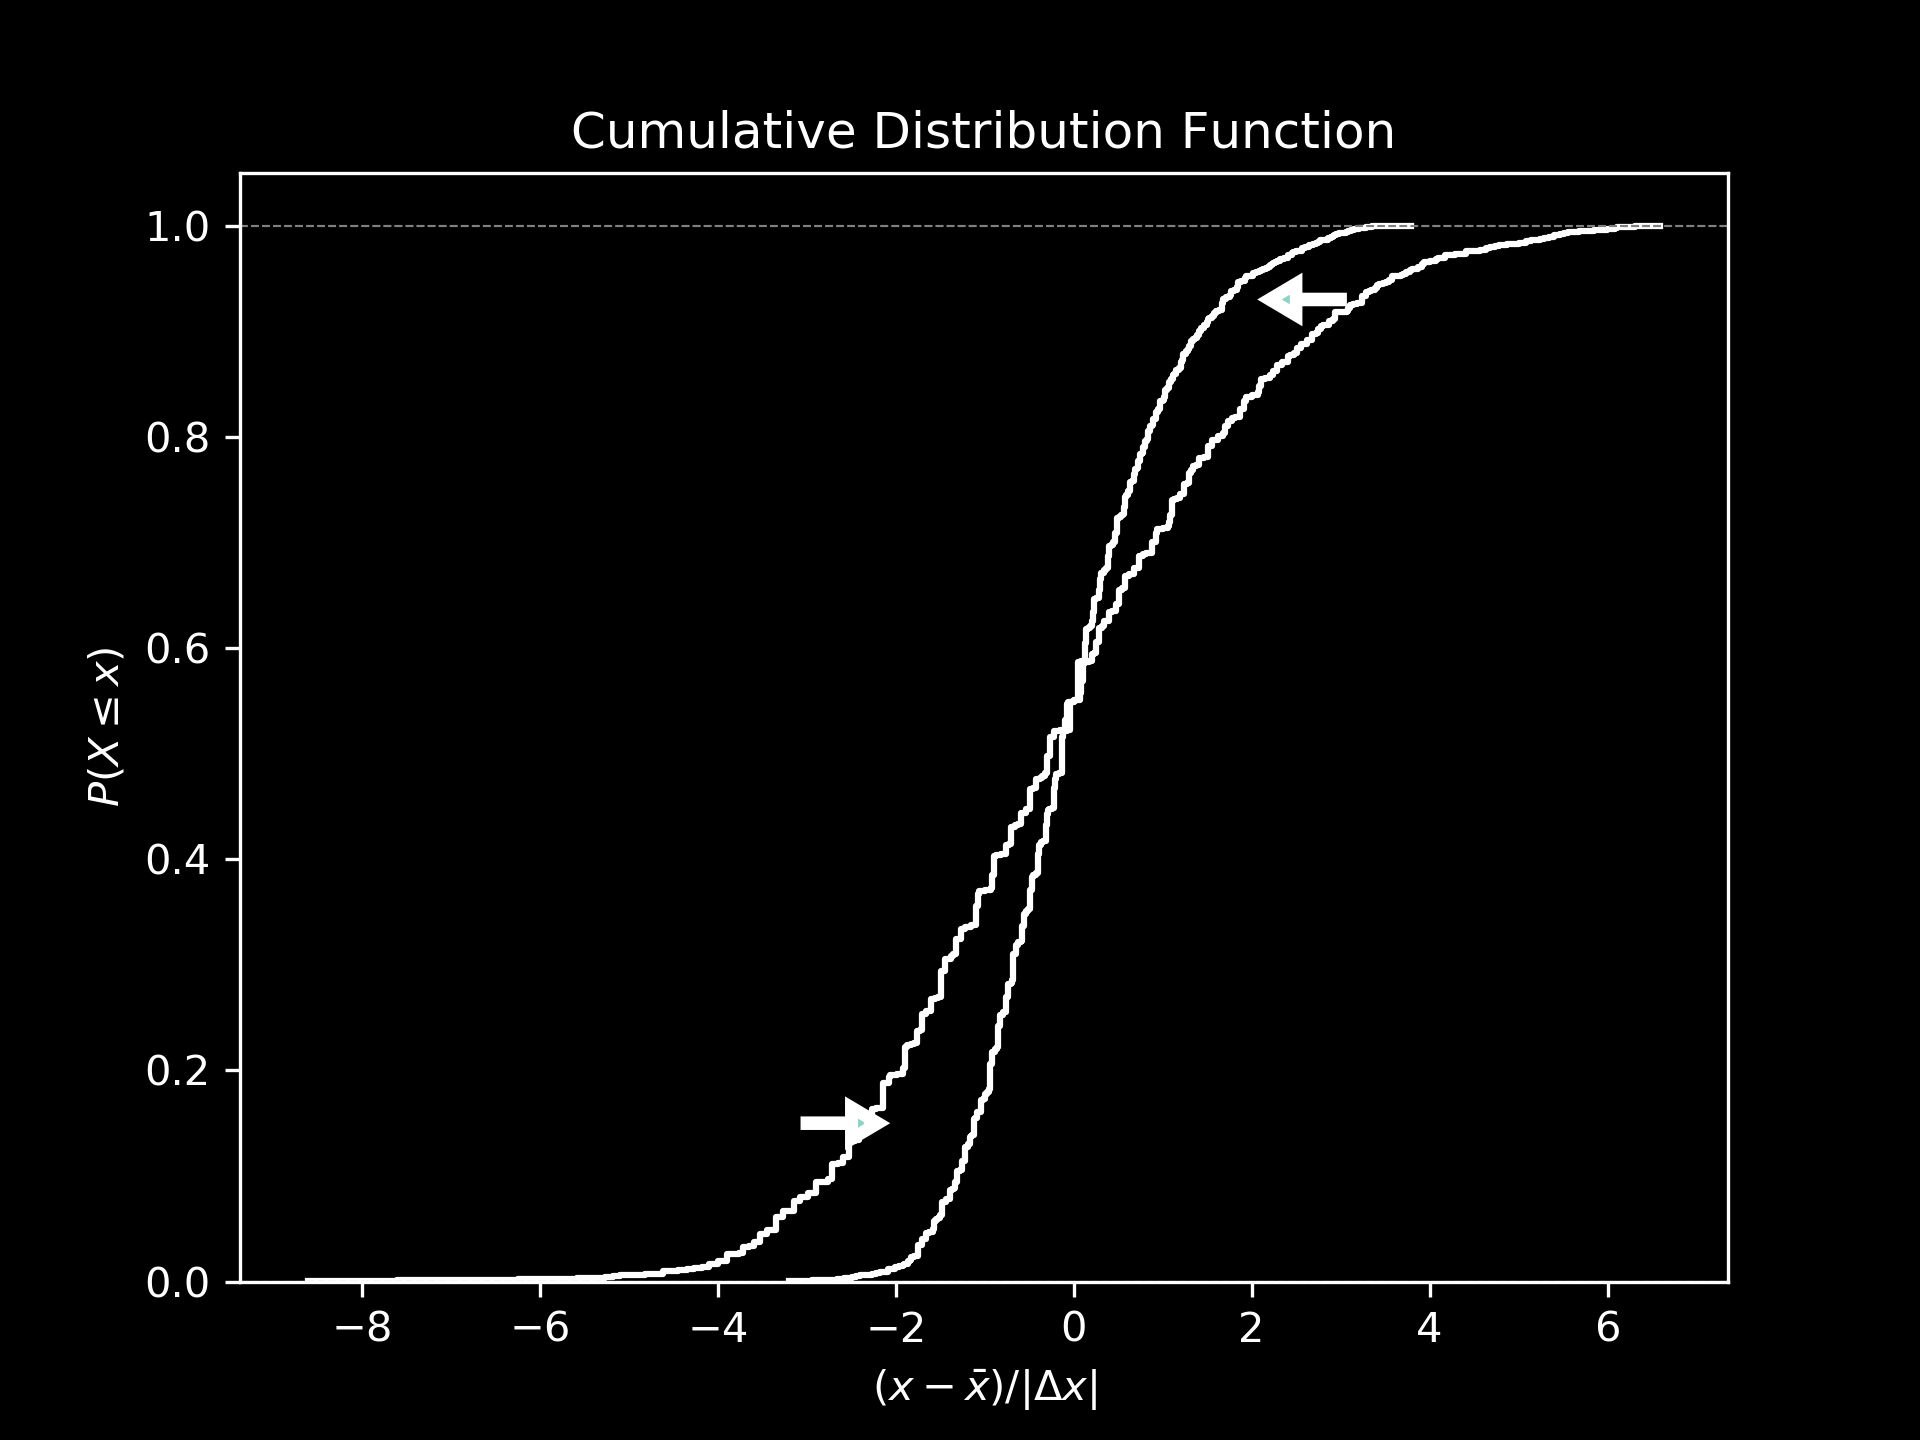
\includegraphics[width=\textwidth]{err_cor1}
\caption{Increasing $C$ narrows the PDF which steepens the CDF}
\label{fig:err_cor1}
\end{figure}

The question obviously is what $C$ is. How does one fit a normal model on a data set with an undefined parameter?
This will be done by minimizing a statistic that represents the sum of squares with a weighting function:
\[
\mathcal{S}(C, \mu, \sigma) = \sum_{i=0}^{n}
\bqty{F_\mathrm{G} (\mathcal{R}_i(C); \mu, \sigma)
  -F(\mathcal{R}_i(C))}^2
\cdot w(\mathcal{R}_i(C); \mu)
\]

This weighting function $w(x)$ is key because it will prioritize the tails of the CDF.
Therefore, it should resemble a parabola, the non-zero center being at the peak of the model $\mu$, rising to the minumum and maximum of the measurement data.
The choice function here is simply a quadratic function:
\[
w(x;\mu, \alpha, \beta)
= \frac{\beta -1}{\alpha ^2}(x-\mu)^2 + 1
\]
where $\beta$ is the ratio between the tail of the differences at $\alpha$ to the center at $\mu$.

Minimizing this $\mathcal{S}$ yields this result shown below in Figure \ref{ref:gauss_ec}.

\begin{figure}[H]
\centering
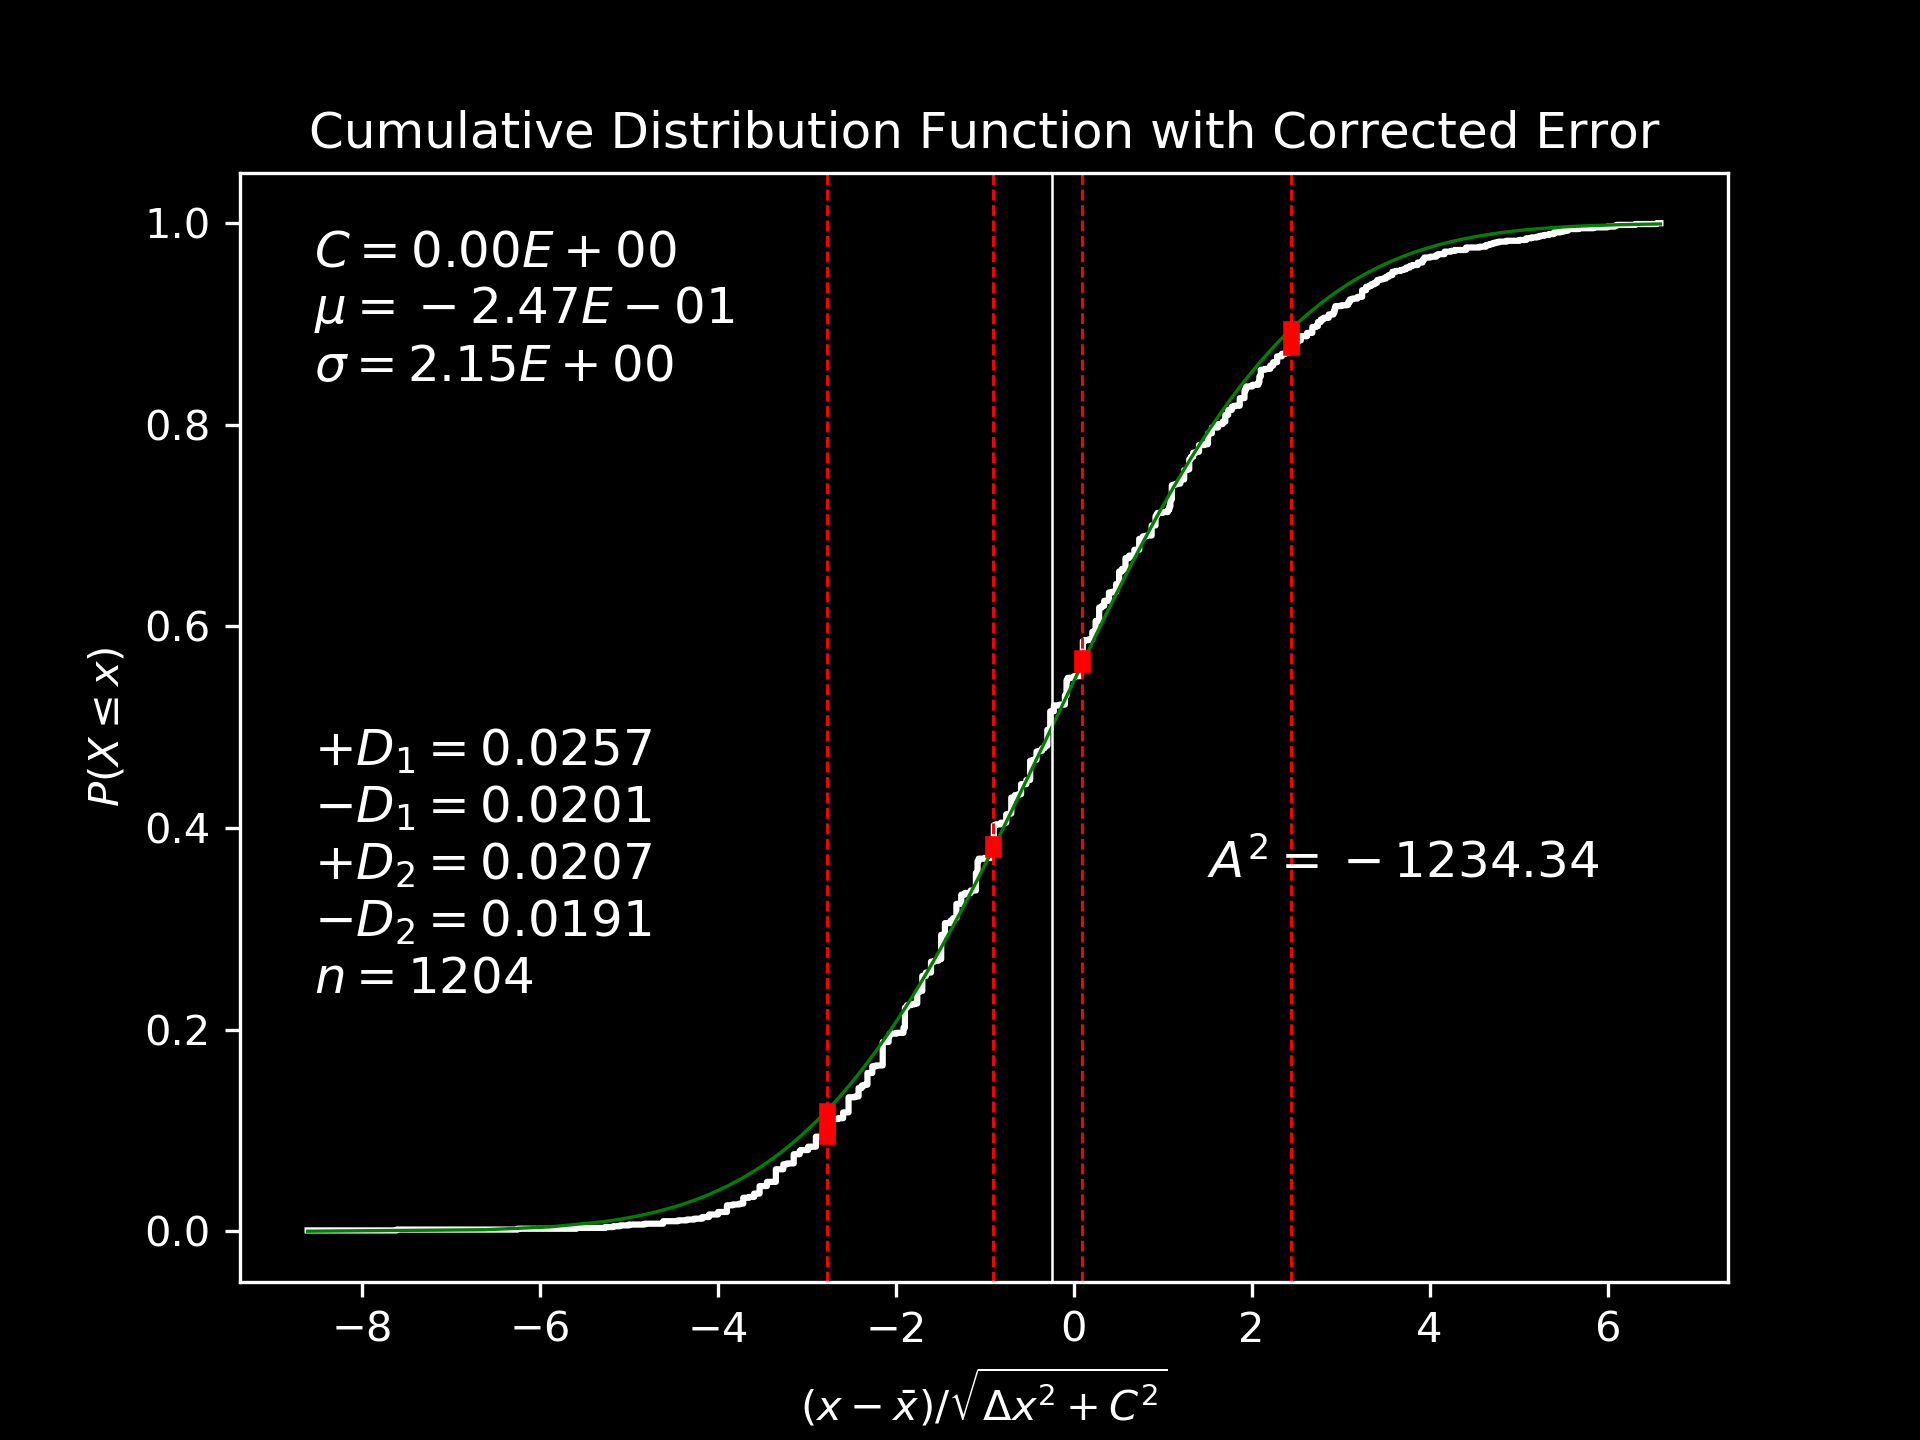
\includegraphics[width=\textwidth]{gauss_ec}
\caption{The KS-tests bring good news.
  The $-D_1$ is smaller bringing the normal model closer to the tail
  $-D_2$ is also smaller; in this case it shows good optimization
}
\label{ref:gauss_ec}
\end{figure}


\section{Correcting for Each Mean Brightness}

Now, to perform this calculation of this correction for all of the 1526 microlensing events observed by the OGLE-IV project in the year 2019. This should bring forth a relationship between the correction term $\mathcal S$ and the non-magnified brightness of the source star.

\par \noindent \textbf{Note}\newline
Unfortunately, computational performance became a major issue at this juncture.
Each iteration involved numerous integrals and a three-dimensional minimization function.
I could not have approximated the integrals because it had devastating effects on the CDF outcomes (like going above 100\%).
The minimization function (for minimizing $\mathcal{S}$) worked on as narrow margins as I could justify.
Still, with a decent computer, each event took between minutes and half-hours.
Not to mention the wild calculation errors (like divide-by-zero errors) that would eliminate many events from the dataset.
Still given enough time and patience, I acquired the following dataset.
I wish I could have dedicated more time into optimizing the script.
Figure \ref{fig:final} was repeated for flux measurements but the lon-awaited result was plagued with too many calculation errors to make any sense of it.

\begin{figure}[H]
\centering
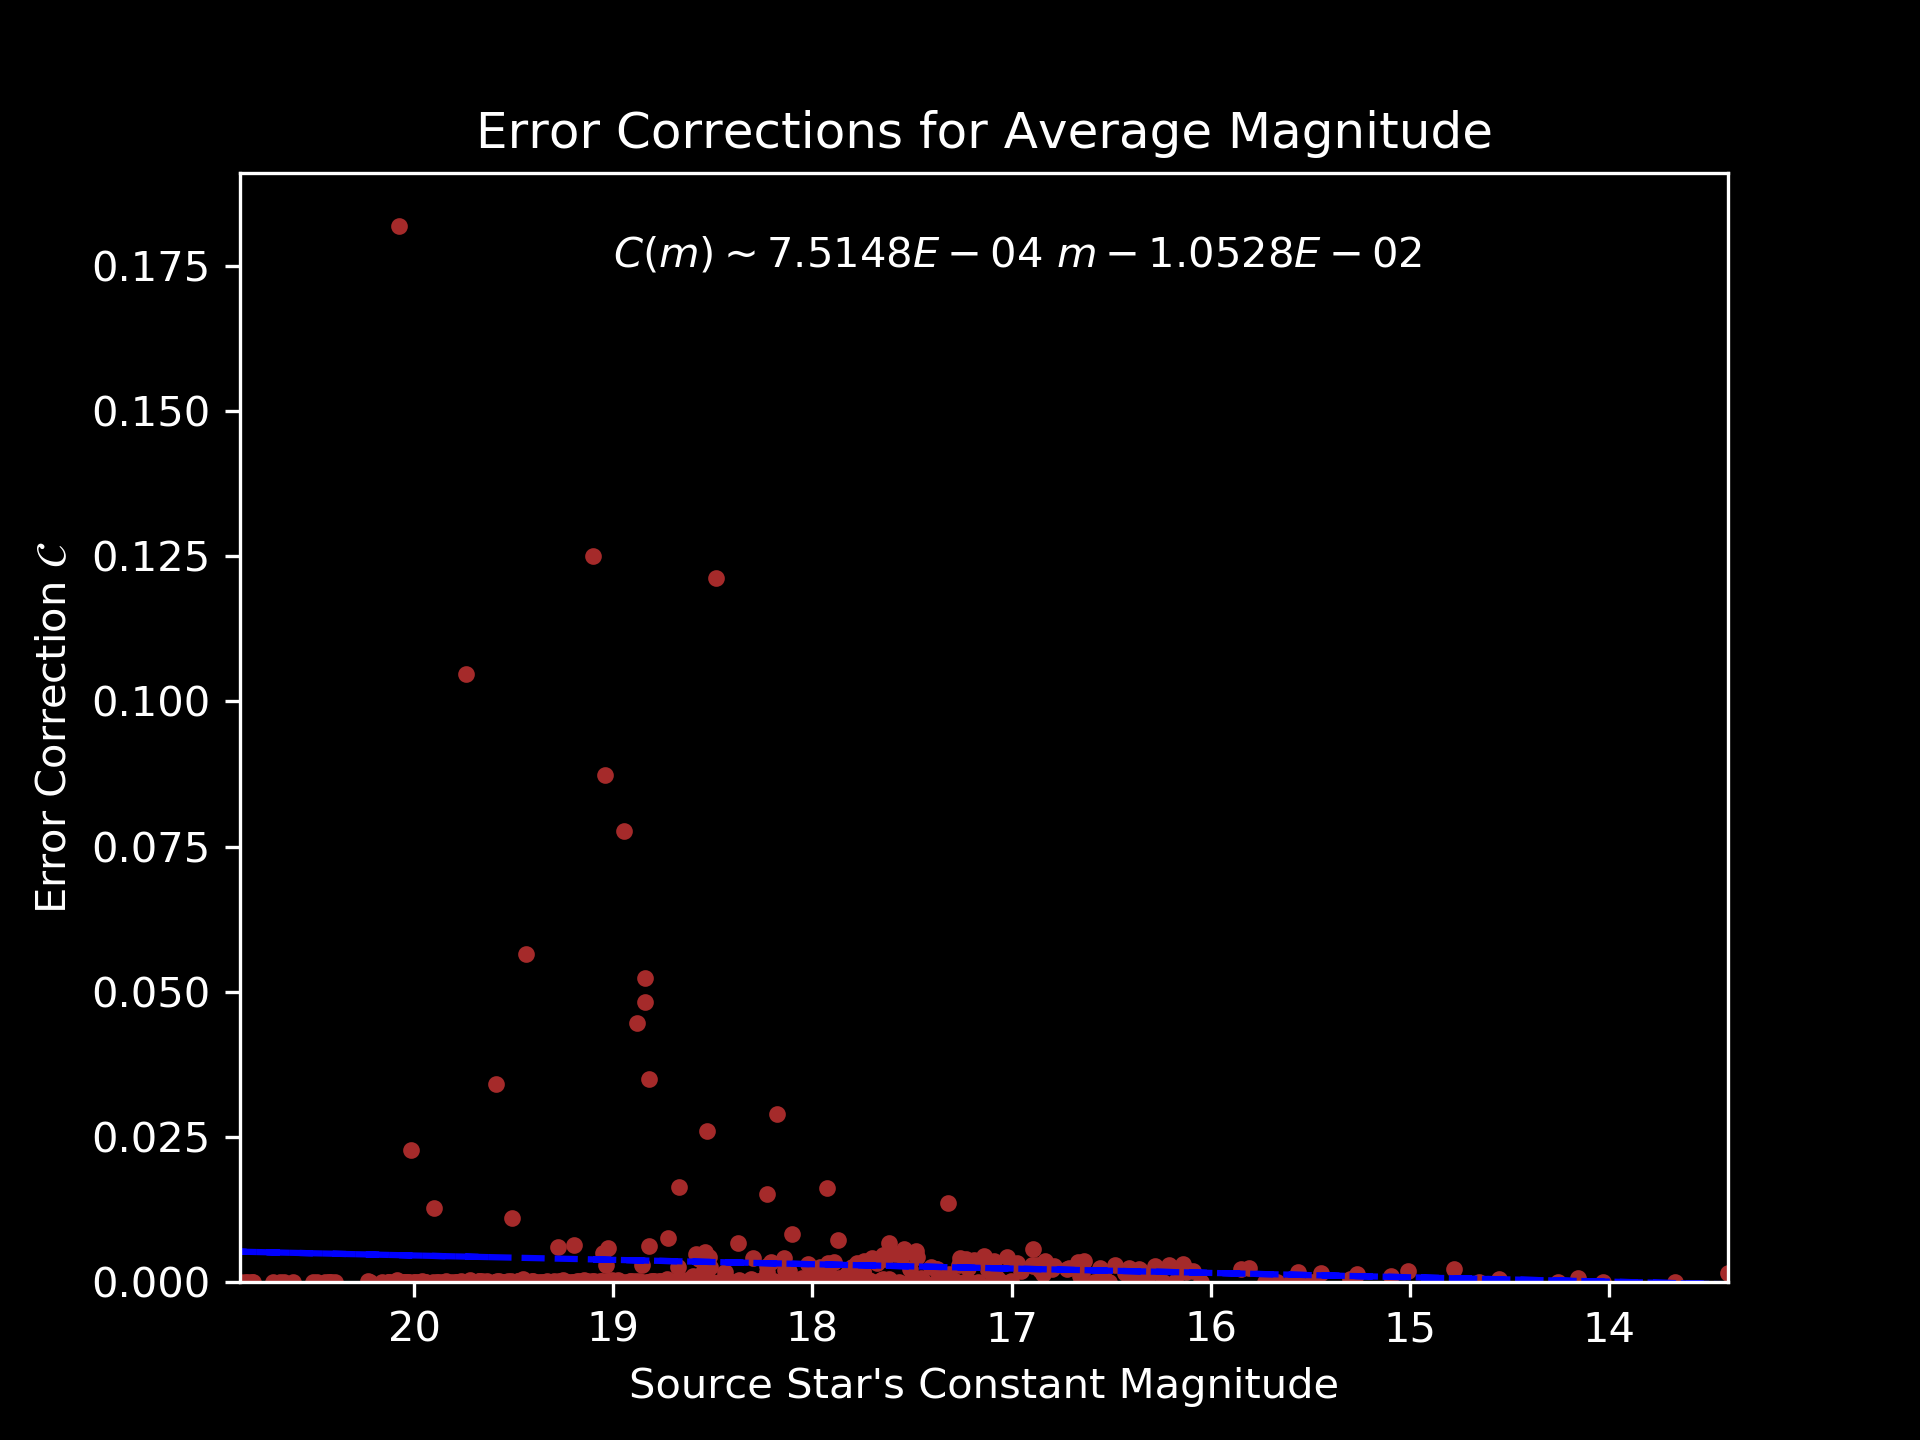
\includegraphics[width=\textwidth]{final}
\caption{Optimized errorbar correction for each event based on the mean magnitude}
\label{fig:final}
\end{figure}

Finally, in Figure \ref{fig:final} we have arrived at a suitable correction term for the error within microlensing photometry parameterized by the non-magnified brightness:
\[
C(m) = (7.515\cdot 10^{-4}) m - (1.053\cdot 10^{-2})
\]

\section{Conclusion}

One can visually measure that the Gaussian / Normal CDF fits the empirical CDF better than those of the Cauchy and student's $t$-distribution.
But the normal fall-off will tend to leave-out legitimate noise deviations.
This mapping will make outliers out of data points that should not be outliers.
So, put forth in this paper are two safer distributions with heavy tails to account for these outcast data points, as well as a correction method for the normal distribution by increasing the error of the data.

By standing up for the deviant noise, we inevitably diminish possible exoplanet detection.
However, identifying more perturbations as noise only increases our certainty about the exoplanetary perturbations that pass more rigorous tests.

\cite{martin}
\cite{paczynski}
\cite{gould_discovering}
\cite{gaudi_parameters}
\cite{PLANET}

\pagebreak
\bibliographystyle{unsrt}
\bibliography{prj}


\end{document}
